% !TEX program = xelatex
% =====================================================================
%  2026 高教社杯全国大学生数学建模竞赛  A 题  药材的烘干问题
%  本文件是论文的唯一样本源。
%  电子版：\documentclass[withoutpreface,bwprint]{cumcmthesis}（即本文件）
%  纸质版：不要手工维护第二份 .tex——用 _polish/build_paper.ps1 派生，
%          它只把下面这一行的 withoutpreface 选项去掉，其余逐字相同，
%          从结构上保证"电子版与纸质版内容完全一致"。
%  编译：  xelatex 论文_最终版.tex   （两遍，生成交叉引用）
% =====================================================================
\documentclass[withoutpreface,bwprint]{cumcmthesis}
\usepackage{amsmath,amssymb}

% ---- 数学字体：让数学模式里的数字与正文的 Times 一致 ----
% 类文件只设了 \setmainfont{Times New Roman}，数学模式仍走 LaTeX 默认的 Computer
% Modern：实测成 PDF 后 $0.9957$ 用的是 CMR12，而紧跟的 241、kg/kg 是 TimesNewRomanPSMT，
% 同一个「2.55 kg/kg」里两种字形挨在一起（指导老师 2026-09-13 书面意见第 2 条）。
% 本机 MiKTeX 未装 newtxmath / unicode-math（且无外网，无法自动安装），改用发行版自带的
% UTM 族（URW Nimbus Roman，Times 的度量兼容体）接管 0--9 十个数字符号。
%
% 为什么只换数字：Times 与 Computer Modern 的数字宽度同为 0.5 em，逐字替换后行宽不变
% （实测页数 71、Overfull 0 均与改前相同）；而 ( ) + - = 两套字体的宽度不同，一并替换会
% 改变断行与页数，收益却只是"括号也换个字体"。数学斜体变量按惯例保留原有字形——本机没有
% Times 的数学斜体字库，强换会引入第三种字形，反而更不统一。
% 必须放在 \AtBeginDocument 里：类文件（经 ctex）在 \begin{document} 处会重新声明数字
% 符号，写在导言区会被它覆盖——这是实测出来的，不要挪回导言区。
\AtBeginDocument{%
  \DeclareSymbolFont{mcmdigits}{OT1}{utm}{m}{n}%
  \DeclareMathSymbol{0}{\mathalpha}{mcmdigits}{`0}%
  \DeclareMathSymbol{1}{\mathalpha}{mcmdigits}{`1}%
  \DeclareMathSymbol{2}{\mathalpha}{mcmdigits}{`2}%
  \DeclareMathSymbol{3}{\mathalpha}{mcmdigits}{`3}%
  \DeclareMathSymbol{4}{\mathalpha}{mcmdigits}{`4}%
  \DeclareMathSymbol{5}{\mathalpha}{mcmdigits}{`5}%
  \DeclareMathSymbol{6}{\mathalpha}{mcmdigits}{`6}%
  \DeclareMathSymbol{7}{\mathalpha}{mcmdigits}{`7}%
  \DeclareMathSymbol{8}{\mathalpha}{mcmdigits}{`8}%
  \DeclareMathSymbol{9}{\mathalpha}{mcmdigits}{`9}%
}

% 插图目录：包内为 figure/（与 fig_core.py 的 FIGDIR 一致）；./fig/ 为备用。
\graphicspath{{../figure/}{./fig/}}

% ---- 中文字形统一：全篇的"加粗"只用一种字形 ----
% 问题（队友 2026-09-13 改动包 §一.3）：ctex 的 windows 方案把加粗映射成 BoldFont=SimHei、
% 把斜体映射成 ItalicFont=KaiTi，于是正文里每个 \textbf{中文} 整段切成黑体（偏深）、注与
% 命题环境的楷体正文切成楷体（偏浅），同一篇论文里"加粗"有两种字形、正文看上去一个字深
% 一个字浅。改法：主中文字体改用 SimSun 的机械加粗（AutoFakeBold），斜体也回到宋体；
% \songti 族（图表题注走它）同样改掉；章节标题原本靠 BoldFont 间接得到黑体，现在显式写
% \heiti，仍然是黑体标题。
\setCJKfamilyfont{zhsong}[AutoFakeBold=3]{SimSun}
\setCJKmainfont[AutoFakeBold=3, ItalicFont={SimSun}]{SimSun}
\ctexset{%
  section/format += \heiti,
  subsection/format += \heiti,
  subsubsection/format += \heiti,
}

\captionsetup{font=small,labelfont=bf,skip=5pt}
\newtheorem{proposition}{命题}
\newtheorem{remark}{注}

% ---- 版面压缩：只动行距与各类间距，不改任何内容、字号与数值 ----
% 行距：模板默认 1.38（12.05 pt 字 / 19.9 pt 行距）。往届获奖论文实测行距区间为
% 15.5~20.5 pt（最紧的两篇约 15.5 pt），此处取 1.10 即 15.9 pt，仍在区间内，
% 相当于 Word 的"单倍行距"，不是把字挤在一起。
\renewcommand*{\baselinestretch}{1.10}
\setlength{\textfloatsep}{5pt plus 2pt minus 2pt}
\setlength{\floatsep}{5pt plus 2pt minus 2pt}
\setlength{\intextsep}{5pt plus 2pt minus 2pt}
\setlength{\emergencystretch}{2.5em}
% 行间公式与题注的留白：\normalsize 会把 \abovedisplayskip 重设为 12 pt，
% 而 \normalsize 在 \begin{document} 时还要再执行一次，故必须放在 AtBeginDocument 里。
\AtBeginDocument{%
  \setlength{\abovedisplayskip}{6pt plus 2pt minus 2pt}%
  \setlength{\belowdisplayskip}{6pt plus 2pt minus 2pt}%
  \setlength{\abovedisplayshortskip}{2pt plus 2pt}%
  \setlength{\belowdisplayshortskip}{4pt plus 2pt minus 2pt}%
  \setlength{\abovecaptionskip}{5pt}%
  \setlength{\belowcaptionskip}{2pt}%
}
% 类文件把 tabular 里的 \arraystretch 硬设成 1.38（与它自带的 \baselinestretch 1.38
% 配套，注释写明"使表格行间距等于正文行间距"）。本文把正文行距收到 1.10，为保持该
% 原意，这里按同一系数重定义 tabular。注意不能用 \AtBeginEnvironment——实测该钩子在
% 类文件那行 \renewcommand 之前执行，会被 1.38 覆盖掉。
\makeatletter
\renewenvironment{tabular}%
  {\bgroup\renewcommand{\arraystretch}{1.10}\mcm@oldtabular}%
  {\mcm@endoldtabular\egroup}
\makeatother
\AtBeginDocument{\hypersetup{pdfauthor={},pdftitle={中药材热风烘干过程的热湿耦合建模与坐标正则化谱方法求解}}}

% ---- 附录源码清单样式：按记号分色 ----
% 附录 C 是几十页连续源码，是评委读代码的唯一入口。原样式里注释是"黑色斜体"、
% 关键字是"黑色加粗"、字符串是类文件自带的紫色，三者与正文字颜色几乎一样（实读 PDF
% 测得只有 #000000 与 #9400d1 两种颜色），扫读时分不出"哪段是说明、哪段是代码"。
% 这里按记号类别分色：注释绿、关键字蓝（加粗）、字符串暗红、行号灰。取值与工作区
% 同题示范论文（参考代码注释/paper_electronic.pdf）实测一致——那套配色在该论文
% 同为 6.6 pt 的代码清单上已被验证可读，属于有据可依而非随手调色。
% 只改颜色，basicstyle 与所有间距参数原样保留，故附录页数与排版不变。
\definecolor{lstcmt}{RGB}{0,128,0}      % 注释
\definecolor{lstkw}{RGB}{0,0,200}       % 关键字
\definecolor{lststr}{RGB}{179,0,0}      % 字符串
\definecolor{lstnum}{RGB}{128,128,128}  % 行号
\lstset{
  basicstyle=\ttfamily\scriptsize,
  breaklines=true,
  columns=flexible,
  keepspaces=true,
  frame=single,
  framexleftmargin=2pt,
  xleftmargin=8pt,
  numbers=left,
  numberstyle=\ttfamily\tiny\color{lstnum},
  numbersep=5pt,
  showstringspaces=false,
  commentstyle=\color{lstcmt},
  keywordstyle=\color{lstkw}\bfseries,
  stringstyle=\color{lststr},
  extendedchars=true,
  literate={ξ}{{$\xi$}}1,
}

% ---- 摘要页的关键词标签：用规范原文的"关键词" ----
% 类文件里 \mcm@cap@keywordsname 默认是"关键字"，是模板的历史写法（往届四届都这么用）。
% 2026 格式规范第三条原文写的是"关键词"，这里改回规范用词。只换这一个词，不动任何版式：
% 该宏在 \keywords 执行时才展开，故在导言区重定义即可，不必改类文件。
\makeatletter
\renewcommand*{\mcm@cap@keywordsname}{关键词}
\makeatother

\title{中药材热风烘干过程的热湿耦合建模与坐标正则化谱方法求解}
\tihao{A}
\baominghao{}
\schoolname{}
\membera{}
\memberb{}
\memberc{}
\supervisor{}
\yearinput{2026}
\monthinput{9}
\dayinput{12}

\begin{document}
\maketitle

% =====================================================================
\begin{abstract}
热风烘干是中药材产地加工中能耗最高、也最易造成药效成分损失的工序，其品质取决于药材
内部温度场与水分场的协同演化。本题的难点有三：圆柱轴心的 $1/r$ 坐标奇异使常规网格
离散复杂化；表面为对流传质而非平衡边界；问题 4 的尺寸收缩构成移动边界，会使固定网格
上的守恒律失真。本文以导热理论、Fick 第二定律与表观体积热容假设为基础，建立中药材
热风烘干过程的圆柱轴对称热湿耦合模型；基于附件 1 的 241 组实测数据建立一阶惯性环境
边界模型，温度与含湿量的拟合决定系数 $R^2$ 分别为 $0.9957$ 与 $0.9901$；控制方程经
坐标正则化 $u=(r/R)^2$ 变换后在 Chebyshev--Gauss--Lobatto 节点上谱配置离散，时间域
采用变阶变步长隐式 BDF 推进。

\textbf{针对问题一：}常物性下热湿两场解耦，难点在于温度场要在指数型环境边界下给出
可核验的基准解。本文将温度场作准静态分解，得到 \textbf{Bessel--Duhamel 级数闭式解}；
水分场在正则坐标上求解。$t=1800$ s 时中心温度、表面温度和表面含水率分别为
$34.0425\,^\circ$C、$37.1989\,^\circ$C 和 $1.5109$ kg/kg，谱解与闭式解的最大差为
$1.14\times10^{-10}$ K。

\textbf{针对问题二：}难点在于物性随温度与含水率同时变化，两场不再解耦。本文将附录 3
的变物性关系代入控制方程，并按附件 1 刻画两阶段烘房环境，通过 $D(C,T_K)$ 与热物性的
相互依赖描述双向耦合。$t=3$ h 时中心温度、中心含水率和表面含水率分别为
$49.9051\,^\circ$C、$1.7673$ kg/kg 和 $1.0083$ kg/kg。

\textbf{针对问题三：}难点在于判据是逐点「处处低于 $0.15$ kg/kg」而非平均值，且最后
干燥点的位置事先未知。本文以全域最大含水率定义终止事件，逐时刻在全部 $N+1$ 个节点上
取极值，得烘干时长 $57.1043$ h（$2.38$ 天），与题目 2—3 天量级独立吻合；若改用截面
平均值判定，会把时长低估 $37.3\%$。

\textbf{针对问题四：}难点在于移动边界会使固定 $r$ 坐标下的守恒律失真。本文引入物质
坐标 $\xi=r/R(t)$，再取 $u=\xi^2$ 消去轴心奇异项，并证明固定 $r$ 坐标下必须保留附加
对流项。采用附录 4 物性并计入实测收缩后得烘干时长 $50.7717$ h；为隔离收缩效应补算
受控基准 $128.9223$ h：物性改变使时长增加 $125.8\%$，而单独考虑尺寸收缩效应时缩短
$60.6\%$，二者方向相反，故问题 3 到问题 4 的 $11.1\%$ 净差异不能归因于收缩。

\textbf{检验与灵敏度：}以闭式解为绝对基准，空间加密至 $N=8$ 即达 $10^{-10}$ K 量级
偏差平台，时间容差收紧至 $10^{-12}$ 时偏差单调降至 $1.1\times10^{-10}$ K；三族独立
离散互差不超过 $2\times10^{-6}$，六种积分器与容差配置给出的烘干时长极差仅 $0.007$ s。
12 组参数扰动表明活化温度 $E$ 最敏感（$\pm2\%$ 使时长变化 $+23.9\%/-18.6\%$）；
环境口径对问题 1 温度场影响达 $0.467\,^\circ$C，而对烘干时长仅 $4.4$ s。

\keywords{热湿耦合；Robin 边界；坐标正则化；谱配置；移动边界；受控对照}
\end{abstract}

% =====================================================================
\section{问题重述}

\subsection{问题背景}

干燥是中药材产地加工与炮制过程中的关键工序，直接决定成品的有效成分保留率、
外观等级与贮藏稳定性。热风烘干因设备简单、成本低而应用最广。该过程分为两个阶段：
先经历「预热平衡阶段」，药材由环境温度被加热到接近烘房温度、内部建立稳定的温度梯度；
随后进入「恒温干燥阶段」，在近似恒定的温湿度环境下水分由内部迁至表面并被气流带走。
工艺参数选择不当会导致干燥过慢（能耗高、周期长）、表面「结壳」（外干内湿）
或温度过高（破坏热敏性成分）。传统的「试错——检测」优化模式周期长、成本高，
近年来针对中药材热风干燥的热湿耦合建模\cite{ao2026modeling}与分段温湿调控
\cite{ju2019stepdown}已有系统研究，为本文提供了对照；
因此有必要用数理模型刻画药材内部温度与水分浓度的时空演化，以预测干燥时长、指导工艺设计。

\subsection{题目条件}

某中药材形状近似为圆柱：长 $L=25$ cm、半径 $R_0=2$ cm。烘干开始时药材温度
$T_0=28\,^\circ$C，水分浓度（干基含水率）$C_0=2.55$ kg/kg。
烘房温度与水分浓度随时间的变化由附件 1 给出（$0\sim14400$ s，每 $60$ s 一点，共 $241$ 点）；
干燥过程中药材半径变化由附件 2 给出（$0\sim259200$ s，每 $1800$ s 一点，共 $145$ 点）。
附录 2--4 分别给出问题 1、问题 2--3、问题 4 所需的物性经验关系。

\subsection{需要解决的问题与量化子任务}

\begin{longtable}{@{}p{1.3cm}p{4.2cm}p{4.1cm}p{4.5cm}@{}}
\toprule
问题 & 输入 & 输出 & 判定标准 \\
\midrule
\endfirsthead
\toprule
问题 & 输入 & 输出 & 判定标准 \\
\midrule
\endhead
一 & 附录 2 物性、附件 1 环境、初值 $(28\,^\circ{\rm C},2.55)$ &
$t=100\sim1800$ s、$r=0\sim2$ cm 的温度与含水率；$1800$ s 内每 $1$ s、每 $0.1$ cm 全结果 &
表~\ref{tab:p1T}、表~\ref{tab:p1C} 保留 4 位小数；\texttt{result1.xlsx} \\
二 & 附录 3 变物性、两阶段工艺 & $3$ h 内每 $0.5$ h 的温度与含水率；全结果 &
表~\ref{tab:p2T}、表~\ref{tab:p2C}；\texttt{result2.xlsx} \\
三 & 同问题二，时间跨度至干燥结束 & 烘干时长；每 $6$ h、每 $0.5$ cm 的含水率 &
\textbf{处处} $C<0.15$ kg/kg；表~\ref{tab:p3}；\texttt{result3.xlsx} \\
四 & 附录 4 物性、附件 2 的 $R(t)$ & 烘干时长；每 $6$ h、每 $0.5$ cm 的含水率 &
同问题三；表~\ref{tab:p4}；\texttt{result4.xlsx} \\
\bottomrule
\end{longtable}
% longtable 在 \begin 时就步进一次 table 计数器（即使没有 \caption）。
% 全文有两张无编号长表（本表与"符号说明"），若不归零，正文第一张真正
% 带编号的表会被编成"表 3"，与文中按结果顺序写的表号整体错开两位。
\setcounter{table}{0}

\subsection{数据探索}

如图~\ref{fig:env} 所示，附件 1 的两个序列均呈明显一阶惯性上升形态：
温度由 $28\,^\circ$C 升至约 $50.2\,^\circ$C 后稳定，含湿量由 $0.01963$ kg/kg
升至约 $0.0509$ kg/kg 后稳定，在 $t\approx4$ h 处进入平台——
这一形态直接决定了后续的环境建模方式（一阶惯性式）与工艺分段（$t=14400$ s）。
附件 2 的半径序列（图~\ref{fig:radius}）单调不增，由 $R(0)=2.000$ cm 迅速下降，
至 $t>207000$ s 后稳定在 $R\approx1.198\sim1.200$ cm（$R/R_0=0.599$），
$90\%$ 的收缩在前 $10$ h 内完成，$|\mathrm{d}R/\mathrm{d}t|$ 在 $t=0$ 处最大。

\begin{figure}[!ht]
\centering

\includegraphics[width=\textwidth]{fig01_env_fit.png}
\caption{附件 1 烘房温度与含湿量的实测序列及一阶惯性拟合}
\label{fig:env}
\end{figure}

\begin{figure}[!ht]
\centering

\includegraphics[width=\textwidth]{fig04_radius.png}
\caption{附件 2 药材半径历史、收缩速率与无量纲收缩比（其中 (b) 为逐区间速率
$|\Delta R/\Delta t|$：实测半径按 $0.001$ cm 的步进下降，半径不变的区间速率为
零，在半对数轴上不绘出）}
\label{fig:radius}
\end{figure}

% =====================================================================
\section{问题分析}

\subsection{总体思路与建模理由链}

本题的核心是一个\textbf{变物性、非线性、带 Robin 边界、且（问题 4 中）求解域随时间收缩}
的轴对称扩散问题。四个问题共用同一套控制方程，差别只在物性关系、环境口径与几何是否收缩。
因此采取「\textbf{一套方程、一套求解框架、四组参数}」的总体思路，把工作量集中在
「把模型建准」与「把数值解算到可信」两件事上。技术路线如图~\ref{fig:flow} 所示。

\begin{figure}[!ht]
\centering

\includegraphics[width=0.92\textwidth]{fig25_flow.png}
\caption{本文技术路线图}
\label{fig:flow}
\end{figure}

\textbf{理由链（以问题 1 为例）}：\emph{机理}——热风对流的边界驱动 + 内部导热/扩散；
\emph{模型形式}——圆柱坐标下的抛物型耦合方程组 + Robin 边界；
\emph{可辨识参数}——$\rho,c_p,k,h,h_m$ 由附录 2 给出，$D(C)$ 由附录 2 的经验式给出，
环境由附件 1 标定，均不含不可辨识参数；
\emph{求解方法}——温度场与水分场解耦 $\Rightarrow$ 温度场可闭式求解（\S\ref{sec:bessel}），水分场用谱配置；
\emph{可验证性}——温度场有闭式解作绝对基准，水分场可用两族离散互证。

\subsection{各问关键点}

\begin{itemize}[leftmargin=1.7em,itemsep=2pt]
\item \textbf{问题 1}：关键在于识别「两场解耦」。附录 2 给的是常数物性、$D$ 只依赖 $C$，
温度方程与水分方程可独立求解；又因烘房温度恰为指数型，温度场可用准静态分解化为闭式级数解。
物理预期为「热快质慢」：$\mathrm{Fo}_T(1800\,{\rm s})=0.760$ 而 $\mathrm{Fo}_D=0.0222$。
\item \textbf{问题 2}：关键是两阶段工艺刻画与变物性耦合。附录 3 的 $D$ 同时依赖 $C$ 与 $T$，
两场真正耦合；温度 $2$ h 内基本平衡，此后药材近似等温体，水分剖面由平缓转为陡峭。
\item \textbf{问题 3}：关键是判据的数学表述与极值点位置。判据是逐点的「处处低于」，
而非平均值；由圆柱几何对称性，中心扩散路径最长，必然是最后干燥点。本文不预设这一点，
而逐时刻对全场节点取最大。
\item \textbf{问题 4}：关键是移动边界。各向同性收缩下若在固定 $r$ 坐标直接套用扩散方程
会漏掉一个对流项，必须改用物质坐标；同时表格列名是「当前物理距离」，
与求解坐标不是一回事，采样须逐时刻换算。
\end{itemize}

% =====================================================================
\section{模型假设}

\begin{enumerate}[leftmargin=1.9em,itemsep=2pt]
\item \textbf{轴对称一维简化}。药材为有限长圆柱，但忽略轴向梯度和端面效应，
温度与干基含水率只依赖 $r$ 和 $t$。长径比 $L/R_0=12.5$，轴向与径向特征时间之比
$(L/R_0)^2=156$；烘房气流沿轴向近似均匀。这一简化的误差在模型评价中单独说明。
\item \textbf{局部热平衡}。骨架与内部水分在同一位置瞬时达到热平衡，用单一温度描述。
题面未给出固液两相换热参数，故采用单温度近似；$\mathrm{Le}=D/\alpha=2.9\times10^{-2}$
仅说明热扩散快于水分扩散，不作为局部热平衡的充分证明。
\item \textbf{干物质不迁移}。干燥中水分迁移，干物质骨架只随整体收缩运动。
固定半径时干物质体积密度 $\rho_d$ 取常数；问题 4 中 $\rho_dR(t)^2$ 沿材料点守恒。
\item \textbf{表面传热传质为对流型}。由 $h$ 与 $h_m$ 控制，且过程中保持常数。
\emph{依据}：题目直接给定 $h=25$ W/(m$^2\cdot$K)、$h_m=8\times10^{-7}$ m/s。
\item \textbf{物性经验关系适用}。三组物性式在其适用区间内成立。因题目未给出标定区间，
本文在 \S\ref{sec:sens} 中对 $E$ 与 $a$ 做 $\pm2\%$ 扰动评估外推风险。
\item \textbf{烘房环境可分段描述}。$0\sim14400$ s 按一阶惯性式变化，其后恒定
（烘房持续排湿）。\emph{依据}：附件 1 在 $t\approx4$ h 达到设定值并稳定。
\item \textbf{收缩各向同性}。同一物质点在任意时刻满足 $r(t)=\xi R(t)$。
\emph{依据}：题目只给出半径方向的收缩数据；\S\ref{sec:shrink} 证明该假设下物质坐标
对流项严格为零。
\item \textbf{采用表观热容近似}。能量方程只保留显热传导，忽略水分迁移携带的显焓、
蒸发潜热和体积变形功。题目未提供含湿焓、汽化潜热与孔隙率等闭合数据，
本文在 \S\ref{sec:eval} 中将其列为适用边界。
\end{enumerate}

% =====================================================================
\section{符号说明}

\begin{center}
\small
\begin{longtable}{@{}p{2.5cm}p{8.4cm}p{3.5cm}@{}}
\toprule
符号 & 含义 & 单位 \\
\midrule
\endfirsthead
\toprule
符号 & 含义 & 单位 \\
\midrule
\endhead
$r$ & 到药材中心的物理距离 & m \\
$R(t)$ & 当前半径（问题 4 变化，其余恒为 $R_0$） & m \\
$R_0,\ L$ & 初始半径、药材长度 & m \\
$T(r,t)$ & 药材温度 & $^\circ$C \\
$C(r,t)$ & 药材干基含水率（kg 水/kg 干物质） & kg/kg \\
$T_{\rm air},C_{\rm air}$ & 烘房温度、空气含湿量 & $^\circ$C, kg/kg \\
$\rho_d$ & 单位当前体积内的干物质质量 & kg/m$^3$ \\
$\rho,\ c_p,\ k$ & 湿物料表观密度、比热容、导热系数 & kg/m$^3$, J/(kg$\cdot$K), W/(m$\cdot$K) \\
$D$ & 以干基含水率梯度为驱动力的有效扩散系数 & m$^2$/s \\
$h,\ h_m$ & 对流换热系数、对流传质系数 & W/(m$^2$K), m/s \\
$\alpha$ & 热扩散率 $k/(\rho c_p)$ & m$^2$/s \\
$\mathrm{Bi},\mathrm{Bi}_m$ & 热/传质 Biot 数 & --- \\
$\mathrm{Fo},\mathrm{Fo}_D$ & 热/传质 Fourier 数 & --- \\
$\mathrm{Le}$ & Lewis 数 $D/\alpha$ & --- \\
$\xi$ & 物质坐标 $r/R(t)$ & --- \\
$u$ & 正则化坐标 $\xi^2$ & --- \\
$T_K$ & Arrhenius 关系使用的绝对温度，$T_K=T+273.15$ & K \\
$E$ & 活化温度参数 $E_a/R_g$（本题为 $3850$ K） & K \\
$a$ & 活化浓度指数 & kg/kg \\
$t_{\rm dry}$ & 烘干时长（处处 $C\le0.15$ 的首达时刻） & s \\
\bottomrule
\end{longtable}
\end{center}
\setcounter{table}{0}   % 同上：把被两张无编号长表吃掉的 table 计数器归零

% =====================================================================
\section{模型的建立}

\subsection{几何简化}

药材为半径 $R_0=2$ cm、长 $L=25$ cm 的圆柱。轴向导热特征时间
$L^2/\alpha\approx3.70\times10^5$ s（约 $4.3$ 天），径向 $R_0^2/\alpha\approx2369$ s，
两者之比恰为 $(L/R_0)^2=156$，相差约 $2.2$ 个数量级；同时烘房气流沿轴向均匀送风。
故端面效应与轴向梯度可以忽略，问题化为轴对称一维径向问题（图~\ref{fig:model}）；
这类圆柱湿物料的热风干燥有成熟的有限差分解与实测对照\cite{hussain}，同一类
「温度场—水分场同时求解」的建模范式在果蔬\cite{wang1995}与中药材\cite{ao2026modeling}
上亦被广泛采用。

\begin{figure}[!ht]
\centering
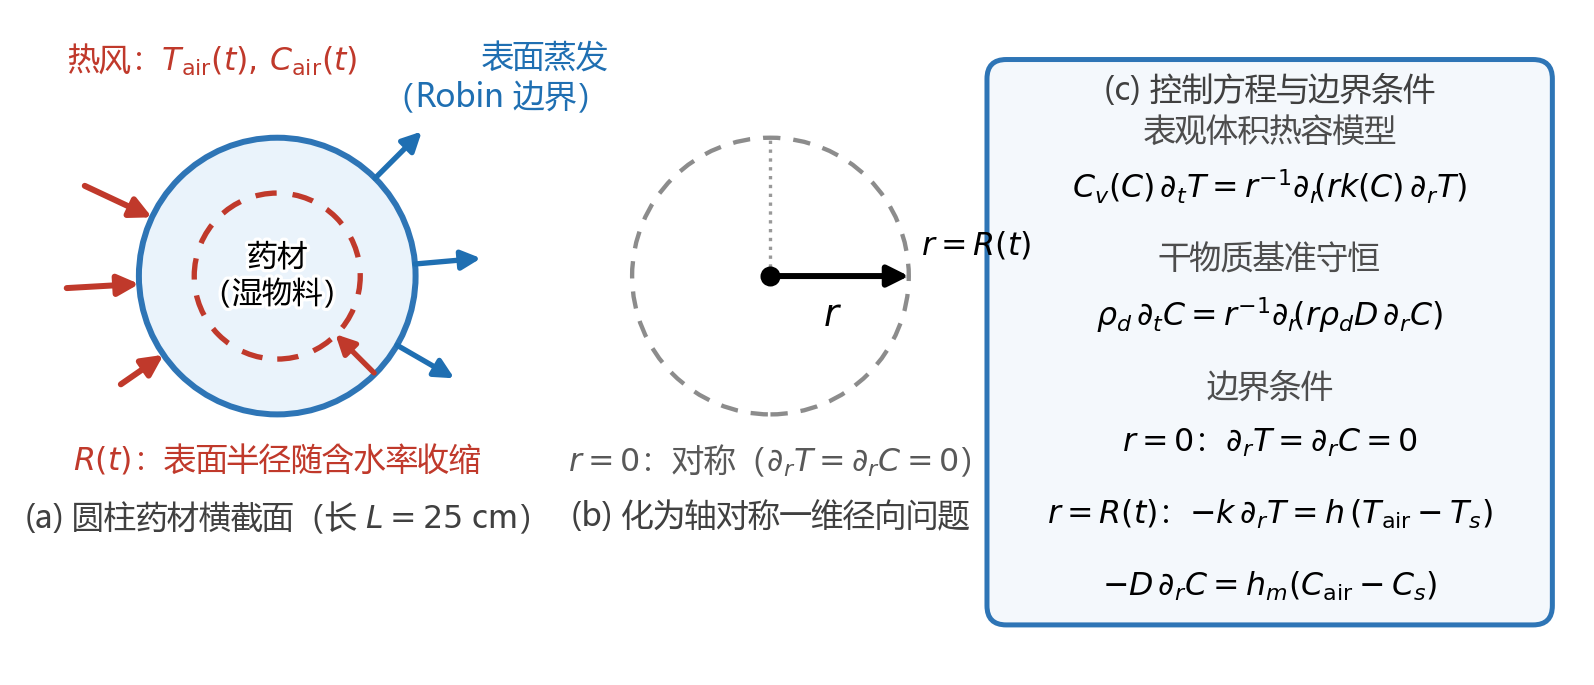
\includegraphics[width=\textwidth]{fig26_model_schematic.png}
\caption{物理模型与坐标系示意图：(a) 圆柱药材横截面，热风对流驱动、表面水分蒸发、
半径随含水率收缩；(b) 取 $1/4$ 截面对称化后的一维径向坐标 $r\in[0,R(t)]$；
(c) 控制方程与 $r=0$ 对称条件、$r=R(t)$ 处 Robin 边界条件}
\label{fig:model}
\end{figure}

\subsection{传热控制方程：表观体积热容模型}

题目给出的 $\rho(C)$、$c_p(C)$ 和 $k(C)$ 视为湿物料的表观热物性，记
$C_v(C)=\rho(C)c_p(C)$。在局部热平衡和显热传导近似下，温度满足
\begin{equation}
C_v(C)\frac{\partial T}{\partial t}
=\frac{1}{r}\frac{\partial}{\partial r}\left(rk(C)\frac{\partial T}{\partial r}\right).
\label{eq:energy}
\end{equation}
式 \eqref{eq:energy} 是以温度为状态变量的表观热容闭合式，不等同于对 $C_vT$ 直接求时间导数。
它在每个时刻根据局部含水率更新 $C_v$ 和 $k$，但不计含湿焓交叉项与蒸发潜热。
若这些热力学数据可获得，则应改用体积焓方程
$\partial_tH(C,T)=r^{-1}\partial_r(rk\partial_rT)-Q_{\rm evap}$。
完备的多孔介质模型还含热湿交叉通量与相变项\cite{luikov}、气相压力与两相动量方程\cite{whitaker}；
题目未给出相应闭合数据，故本文只取其对 Fourier--Fick 极限的简化形式。

\subsection{传质控制方程：干物质基准守恒}

以干基含水率 $C$ 为变量，单位当前体积内的水分质量为 $\rho_dC$，相对于干物质骨架的
水分通量取为 $j_r=-\rho_dD(C,T_K)\partial_rC$。问题 1--3 的半径固定，干物质骨架
不发生宏观运动，且 $\rho_d$ 在求解域内取常数。环形壳层的水分衡算为
\[
\rho_d\frac{\partial C}{\partial t}
=\frac{1}{r}\frac{\partial}{\partial r}
\left(r\rho_dD\frac{\partial C}{\partial r}\right).
\]
约去常数 $\rho_d$ 后得到
\begin{equation}
\frac{\partial C}{\partial t}
=\frac{1}{r}\frac{\partial}{\partial r}\left(rD(C,T_K)\frac{\partial C}{\partial r}\right).
\label{eq:mass}
\end{equation}
这里的 $\rho_d$ 是干物质体积密度，不与经验湿物料密度 $\rho(C)/(1+C)$ 混用；
$D$ 被解释为以干基含水率梯度为驱动力的有效扩散系数。若令 $\rho_d$ 随空间或时间变化，
则必须保留其在守恒式中的位置，不能直接约去。

\subsection{边界条件与初始条件}

中心对称：$\partial_rT(0,t)=\partial_rC(0,t)=0$。
表面 Robin 条件（$r=R$）：
\begin{equation}
-k\left.\frac{\partial T}{\partial r}\right|_{r=R}=h(T_s-T_{\rm air}(t)),
\qquad
-D\left.\frac{\partial C}{\partial r}\right|_{r=R}=h_m(C_s-C_{\rm air}(t)),
\label{eq:robin}
\end{equation}
其中 $T_s=T(R,t)$、$C_s=C(R,t)$。$C_s-C_{\rm air}$ 是题目给定经验边界中的
有效传质驱动力；固相干基含水率与气相含湿量的分母基准不同，本式不表示二者满足直接相平衡。
题面未给出吸附等温线或界面分配系数，故不再增加无法标定的界面参数。初始条件为
$T(r,0)=28\,^\circ$C，$C(r,0)=2.55$ kg/kg。

\subsection{烘房环境数据的标定}
\label{sec:calib}

附件 1 是带噪实测序列，直接作边界会把测量噪声注入解。由图~\ref{fig:env} 的一阶惯性形态，
先作一阶惯性拟合，\textbf{初值固定为实测初值}：
\begin{equation}
T_{\rm air}(t)=T_{\rm set}-(T_{\rm set}-28)e^{-t/\tau_T},
\qquad
C_{\rm air}(t)=C_{\rm set}-(C_{\rm set}-0.01963)e^{-t/\tau_C}.
\label{eq:ambient}
\end{equation}
用 Levenberg--Marquardt 非线性最小二乘（初值固定，每式只有 $2$ 个自由参数）得

\begin{table}[!ht]
\centering
\small
\caption{烘房环境一阶惯性标定结果}
\begin{tabular}{@{}lcccc@{}}
\toprule
参数 & 拟合值 & 标准误 & RMSE & $R^2$ \\
\midrule
$T_{\rm set}$ / $^\circ$C & 50.2121 & 0.0303 & \multirow{2}{*}{0.336 $^\circ$C} & \multirow{2}{*}{0.9957} \\
$\tau_T$ / s & 1877.49 & 12.74 & & \\
$C_{\rm set}$ / (kg/kg) & 0.050908 & $9.3\times10^{-5}$ & \multirow{2}{*}{$8.1\times10^{-4}$} & \multirow{2}{*}{0.9901} \\
$\tau_C$ / s & 2776.34 & 31.71 & & \\
\bottomrule
\end{tabular}
\end{table}

计算中把标定参数按其有效位数取用（$T_{\rm set}=50.212$、$\tau_T=1877.5$、$\tau_C=2776.3$）。
该取舍在 $T(R,1800\,{\rm s})$ 上仅造成约 $6\times10^{-5}\,^\circ$C 的变化，
比标定标准误小三个数量级。

工艺分段：由附件 1 可见烘房在 $t\approx4$ h 达到设定值并稳定，故取
\begin{equation}
(T_{\rm air},C_{\rm air})=
\begin{cases}
\text{式}\eqref{eq:ambient}, & 0\le t\le14400\ {\rm s},\\[2pt]
(50.212\,^\circ{\rm C},\ 0.050908\ {\rm kg/kg}), & t>14400\ {\rm s}.
\end{cases}
\label{eq:stage}
\end{equation}

该分段在 $t=14400$ s 处不连续：一阶惯性式在该点的取值为 $50.2016\,^\circ$C 与
$0.050733$ kg/kg，与设定值分别相差 $0.0104\,^\circ$C 与 $1.75\times10^{-4}$ kg/kg。
相对于全程变化量（温度约 $22\,^\circ$C、含湿量约 $0.031$ kg/kg）分别只有
$5\times10^{-4}$ 与 $6\times10^{-3}$，也小于环境拟合自身的 RMSE，故直接切换到设定值
不会带来可见误差。若需严格连续，则应把分段点后移，或对惯性式作尾部截断。

\subsection{物性经验关系与量纲检查}

\begin{table}[!ht]
\centering
\small
\caption{三组物性经验关系（附录 2--4）}
\begin{tabular}{@{}lccc@{}}
\toprule
 & 问题 1（附录 2） & 问题 2、3（附录 3） & 问题 4（附录 4） \\
\midrule
$\rho$ / (kg/m$^3$) & $820$ & $650+128C$ & $760+90C$ \\
$c_p$ / (J/(kg$\cdot$K)) & $2600$ & $1450+2736\dfrac{C}{C+1}$ & $1850+2150\dfrac{C}{C+1}$ \\
$k$ / (W/(m$\cdot$K)) & $0.36$ & $0.21+0.38\dfrac{C}{C+1}$ & $0.12+0.20\dfrac{C}{C+1}$ \\
$D$ / (m$^2$/s) & $7\times10^{-9}e^{-0.89/C}$ &
$2.4\times10^{-3}e^{-0.45/C}e^{-3850/T_K}$ &
$4.2\times10^{-4}e^{-0.30/C}e^{-3850/T_K}$ \\
\bottomrule
\end{tabular}
\end{table}

$e^{-3850/T_K}$ 为 Arrhenius 因子，对应活化能 $E_a=3850R_g=32.0$ kJ/mol。
量纲检查：$3850$ K 量纲为温度，$T_K=T+273.15$ 须取绝对温度；
$a$ 与 $C$ 同量纲（kg/kg），故 $a/C$ 无量纲。

\begin{remark}[经验式的读法自检]
附录 2 写成 $D=7\times10^{-9}e^{-0.89/C}$，指数部分有两种读法。
若读作 $e^{-0.89C}$，则 $C$ 由 $2.55$ 降到 $0.15$ 时 $D$ 反而\textbf{增大} $8.5$ 倍
（$e^{-0.89\times0.15}/e^{-0.89\times2.55}=8.47$），与「越干越难扩散」的降速干燥事实矛盾；
读作 $e^{-0.89/C}$ 时 $D$ 下降 $266$ 倍，正是降速干燥所要求的。
附录 3 同判：$e^{-0.45/C}$ 使 $D$ 由 $C=2.55$ 到 $C=0.15$ 下降 $16.8$ 倍。
故三个 $D$ 式中的指数一律读作 $e^{-a/C}$。

温度取绝对温度：由附录 3 在 $C=2.55$、$T=50\,^\circ$C 处得 $D=1.347\times10^{-8}$ m$^2$/s，
与已有中药材干燥实测的有效水分扩散系数 $3.90\times10^{-9}\sim2.04\times10^{-8}$ m$^2$/s\cite{zhangwp}
属同一数量级（该系数随材料、尺寸与干燥方式变化，比较仅用于量级校验）；
若把 $T$ 误按摄氏度代入，$e^{-3850/50}\approx0$，$D$ 退化为零，显然不合理。
\end{remark}

\subsection{无量纲分析}

定义 $\mathrm{Bi}=hR_0/k$、$\mathrm{Bi}_m=h_mR_0/D$、
$\mathrm{Fo}=\alpha t/R_0^2$、$\mathrm{Le}=D/\alpha$。取问题 1 参数：
$\alpha=1.6886\times10^{-7}$ m$^2$/s，$\mathrm{Bi}=1.3889$，
$D(C_0)=4.9377\times10^{-9}$ m$^2$/s，$\mathrm{Bi}_m=3.2404$，$\mathrm{Le}=2.9\times10^{-2}$，
于是 $\mathrm{Fo}_T(1800\,{\rm s})=0.760$、$\mathrm{Fo}_D(1800\,{\rm s})=0.0222$
（图~\ref{fig:dimless}）。两条先验结论：其一 $\mathrm{Fo}_D\ll\mathrm{Fo}_T$，
温度先于水分达到准平衡；其二 $\mathrm{Bi}_m$ 量级为 $1$，
内部扩散阻力与外部对流传质阻力相当，必须保留 Robin 条件而不能把表面当作平衡边界。

\begin{figure}[!ht]
\centering

\includegraphics[width=\textwidth]{fig05_dimensionless.png}
\caption{无量纲分析：Fourier 数、特征时间尺度与无量纲判据}
\label{fig:dimless}
\end{figure}

\subsection{新方法的出发点：坐标正则化}
\label{sec:reg}

\subsubsection{轴心奇异结构}

把式 \eqref{eq:energy}、\eqref{eq:mass} 的算子展开：
\begin{equation}
\mathcal{L}\phi:=\frac{1}{r}\frac{\partial}{\partial r}\left(ra\frac{\partial\phi}{\partial r}\right)
=a\frac{\partial^2\phi}{\partial r^2}+\frac{a}{r}\frac{\partial\phi}{\partial r}
+\frac{\partial a}{\partial r}\frac{\partial\phi}{\partial r},
\end{equation}
第二项含 $1/r$。虽然由对称性 $\partial_r\phi(0)=0$ 使极限有限，但离散格式必须显式处理
这一奇异——常规节点中心有限体积要把最内控制体取成 $[0,h/2]$ 并令其测度为 $h^2/8$，
界面差分还要借助对称性做单侧外推。这正是常规 $r$ 坐标离散的主要复杂度来源。

\subsubsection{正则化变换}

\begin{proposition}[圆柱 Laplace 算子的正则化]
令 $u=\xi^2=(r/R)^2$，则对任意光滑 $a(u)$，
\begin{equation}
\frac{1}{r}\frac{\partial}{\partial r}\left(ra\frac{\partial\phi}{\partial r}\right)
=\frac{4}{R^2}\frac{\partial}{\partial u}\left(ua\frac{\partial\phi}{\partial u}\right),
\label{eq:reg}
\end{equation}
且右端在 $u=0$ 取有限值 $\partial_u(ua\partial_u\phi)|_{u=0}=a(0)\partial_u\phi(0)$。
\end{proposition}
\noindent\textbf{证明.}\ 
由 $r=R\sqrt u$ 得 $\partial r/\partial u=R/(2\sqrt u)$，故
$\partial/\partial r=\dfrac{2\sqrt u}{R}\dfrac{\partial}{\partial u}$。逐步计算：
\[
a\frac{\partial\phi}{\partial r}=a\frac{2\sqrt u}{R}\frac{\partial\phi}{\partial u},
\qquad
ra\frac{\partial\phi}{\partial r}=R\sqrt u\cdot a\cdot\frac{2\sqrt u}{R}\frac{\partial\phi}{\partial u}
=2ua\frac{\partial\phi}{\partial u},
\]
\[
\frac{\partial}{\partial r}\left(2ua\frac{\partial\phi}{\partial u}\right)
=\frac{2\sqrt u}{R}\frac{\partial}{\partial u}\left(2ua\frac{\partial\phi}{\partial u}\right),
\]
\[
\frac{1}{r}\frac{\partial}{\partial r}\left(ra\frac{\partial\phi}{\partial r}\right)
=\frac{1}{R\sqrt u}\cdot\frac{2\sqrt u}{R}\cdot
\frac{\partial}{\partial u}\left(2ua\frac{\partial\phi}{\partial u}\right)
=\frac{4}{R^2}\frac{\partial}{\partial u}\left(ua\frac{\partial\phi}{\partial u}\right).
\]
正则性由 $\partial_u(ua\partial_u\phi)=a\partial_u\phi+u\partial_u(a\partial_u\phi)$
在 $u=0$ 处第二项为零立即得到。


因此两个控制方程在 $u\in(0,1)$ 上统一写成
\begin{equation}
\boxed{\;
\frac{\partial C}{\partial t}=\frac{4}{R^2}\frac{\partial}{\partial u}\left(uD\frac{\partial C}{\partial u}\right),
\qquad
\rho c_p\frac{\partial T}{\partial t}=\frac{4}{R^2}\frac{\partial}{\partial u}\left(uk\frac{\partial T}{\partial u}\right).
\;}
\label{eq:gov}
\end{equation}
在 $u=1$ 处 $\partial_r=2\partial_u/R$，Robin 条件化为
\begin{equation}
2D\left.\frac{\partial C}{\partial u}\right|_{u=1}=h_mR(C_{\rm air}-C_1),
\qquad
2k\left.\frac{\partial T}{\partial u}\right|_{u=1}=hR(T_{\rm air}-T_1).
\label{eq:bc_u}
\end{equation}
$u=0$ 处采用正则解类：$\partial_uC$ 与 $\partial_uT$ 有界，于是
$\partial_rC=2\sqrt{u}\,\partial_uC/R$ 和 $\partial_rT=2\sqrt{u}\,\partial_uT/R$ 自动趋于零。
离散时直接在端点配置正则化方程，不再增加与正则性重复的独立边界值。

\subsubsection{为什么谱方法在 $u$ 坐标下成立}

\begin{proposition}[解析性]
设 $C(\xi,t)$ 关于 $\xi$ 为偶函数且解析，则 $C$ 作为 $u=\xi^2$ 的函数在 $[0,1]$ 上解析。
\end{proposition}
\noindent\textbf{证明.}\ 
偶解析函数有 Taylor 展开 $C(\xi)=\sum_{k\ge0}a_{2k}\xi^{2k}$，代入 $u=\xi^2$ 即得
$C(u)=\sum_{k\ge0}a_{2k}u^k$。

具体地，线性问题特征函数 $J_0(\beta_nr/R)=\sum_{k\ge0}\frac{(-1)^k}{k!k!}
\left(\frac{\beta_n^2}{4}\right)^ku^k$ 是 $u$ 的整函数。
故在 Chebyshev--Gauss--Lobatto 节点上做配置可获得谱精度（图~\ref{fig:utrans}）。本文选择 $u$ 而非 $\xi$
作为配置变量，是为了把偶对称结构直接编码到坐标中并简化轴心端点处理；
在 $\xi$ 坐标上显式施加对称条件同样可以构造谱方法，因此这里不把该变换表述为唯一选择。

\begin{figure}[!ht]
\centering

\includegraphics[width=\textwidth]{fig06_u_transform.png}
\caption{坐标正则化：常规 $r$ 坐标与正则化坐标 $u=\xi^2$ 的节点分布对比}
\label{fig:utrans}
\end{figure}

% =====================================================================
\section{问题一：预热平衡阶段的求解}

\subsection{温度场的闭式解（Bessel--Duhamel 展开）}
\label{sec:bessel}

问题 1 的 $\rho,c_p,k$ 为常数、$D$ 只依赖 $C$，故两场\textbf{完全解耦}；
又环境为指数型式 \eqref{eq:ambient}，温度场可\textbf{不离散}地闭式求出。

记 $A=T_{\rm set}-28$，$T_{\rm air}(t)=T_{\rm set}-Ae^{-t/\tau_T}$，
令 $w(r,t)=T(r,t)-T_{\rm air}(t)$。由于 $T_{\rm air}$ 与 $r$ 无关，$\nabla^2T=\nabla^2w$，于是
\begin{equation}
\frac{\partial w}{\partial t}=\alpha\nabla^2w-\frac{A}{\tau_T}e^{-t/\tau_T},
\qquad
-k\left.\frac{\partial w}{\partial r}\right|_{r=R}=hw(R,t),
\qquad
w(r,0)=0 .
\label{eq:w}
\end{equation}
（初值：$w(r,0)=28-(T_{\rm set}-A)=0$。）

\textbf{准静态分解}。设 $w=W(r)e^{-t/\tau_T}+\hat w(r,t)$，代入式 \eqref{eq:w}：
\[
\frac{\partial\hat w}{\partial t}=\alpha\nabla^2\hat w
+e^{-t/\tau_T}\left[\alpha\nabla^2W+\frac{W}{\tau_T}-\frac{A}{\tau_T}\right].
\]
令中括号为零，则 $\hat w$ 满足齐次热方程，$W$ 满足
\begin{equation}
\nabla^2W+\kappa^2W=\kappa^2A,\quad \kappa^2:=\frac{1}{\alpha\tau_T},
\qquad
-kW'(R)=hW(R),
\label{eq:Wode}
\end{equation}
且 $\hat w(r,0)=-W(r)$。式 \eqref{eq:Wode} 通解为 $W=A+BJ_0(\kappa r)+D_0Y_0(\kappa r)$；
由 $r=0$ 处有界性去掉 $Y_0$，常数解 $A$ 是 $\kappa^2A$ 的特解。代入 Robin 条件
（$\frac{\rm d}{{\rm d}r}J_0(\kappa r)=-\kappa J_1(\kappa r)$）得
\begin{equation}
\boxed{\;W(r)=A+BJ_0(\kappa r),\qquad
B=\frac{hA}{k\kappa J_1(\kappa R)-hJ_0(\kappa R)},\qquad
\kappa=\frac{1}{\sqrt{\alpha\tau_T}}.\;}
\label{eq:W}
\end{equation}

\textbf{特征值问题}。$\hat w$ 满足齐次热方程与齐次 Robin 条件，分离变量得
\begin{equation}
\phi_n(r)=J_0\!\left(\frac{\beta_nr}{R}\right),
\qquad
\beta_nJ_1(\beta_n)=\mathrm{Bi}J_0(\beta_n),
\qquad
\gamma_n=\frac{\alpha\beta_n^2}{R^2},
\label{eq:eig}
\end{equation}
在权 $r$ 下正交：$\int_0^Rr\phi_n\phi_m{\rm d}r=\frac{R^2}{2}
[J_0^2(\beta_n)+J_1^2(\beta_n)]\delta_{nm}$（该展开属经典导热解析框架\cite{carslaw}），
本文据此对指数型环境边界作准静态分解。

\textbf{展开系数}。设 $\hat w=\sum_nb_n\phi_ne^{-\gamma_nt}$，则 $b_n$ 是 $-W$ 的带权投影系数。
由 Green 恒等式和 Robin 边界条件可得（完整推导见附录~\ref{app:besselcoef}的式~\eqref{eq:bn}）
\begin{equation}
\boxed{\begin{aligned}
b_n&=\frac{A\kappa^2N_n}{(\beta_n^2/R^2)-\kappa^2},\\
N_n&=\frac{2J_1(\beta_n)}{\beta_n[J_0^2(\beta_n)+J_1^2(\beta_n)]},\\
T(r,t)&=T_{\rm air}(t)+W(r)e^{-t/\tau_T}
+\sum_{n\ge1}b_nJ_0\!\left(\frac{\beta_nr}{R}\right)e^{-\gamma_nt}.
\end{aligned}}
\label{eq:Tsol}
\end{equation}

\textbf{一致性自检}：$t=0$ 时 $T_{\rm air}(0)=28$ 且
$W(r)+\sum_nb_n\phi_n(r)=W(r)-W(r)=0$，故 $T(r,0)\equiv28$；$t\to\infty$ 时 $T\to T_{\rm set}$。
\textbf{收敛速度}：$t=1800$ s 时 $\gamma_nt$ 依次为 $1.529,13.191,39.483,80.742$，
即 $n\ge2$ 项已压至 $e^{-13.2}\approx1.8\times10^{-6}$ 以下（图~\ref{fig:bessel}），
故式 \eqref{eq:Tsol} 的前两项已满足本文四位小数的报告精度；高精度验证仍按程序保留完整截断级数。

计算参数、前四个特征根与展开系数列于附录~\ref{app:besselcoef}，并由图~\ref{fig:bessel}给出衰减核验。

\begin{figure}[!ht]
\centering

\includegraphics[width=\textwidth]{fig10_bessel_coef.png}
\caption{Bessel--Duhamel 展开：系数 $b_n$ 的衰减与各阶衰减因子 $\gamma_nt$}
\label{fig:bessel}
\end{figure}

\subsection{水分场的谱配置求解}

水分方程由式 \eqref{eq:gov} 给出，初值 $C\equiv2.55$，表面通量由式 \eqref{eq:bc_u} 给出。
注意初值 $C_s=2.55$ 而 $C_{\rm air}=0.0196$，存在初值跳跃，须用自适应的首步抑制振荡。
空间离散见 \S\ref{sec:numeric}。

\subsection{求解结果}

\begin{table}[!ht]
\centering
\small
\caption{30 分钟内药材的温度（单位：$^\circ$C）}
\label{tab:p1T}
\begin{tabular}{@{}lccccc@{}}
\toprule
时间/s & $r=0$ & $r=0.5$ cm & $r=1.0$ cm & $r=1.5$ cm & $r=2.0$ cm \\
\midrule
100  & 28.0001 & 28.0005 & 28.0054 & 28.0425 & 28.2219 \\
300  & 28.0500 & 28.0776 & 28.1857 & 28.4550 & 29.0261 \\
600  & 28.5456 & 28.6438 & 28.9618 & 29.5667 & 30.5576 \\
900  & 29.5568 & 29.7074 & 30.1740 & 30.9976 & 32.2359 \\
1200 & 30.9069 & 31.0882 & 31.6397 & 32.5824 & 33.9433 \\
1500 & 32.4397 & 32.6353 & 33.2248 & 34.2150 & 35.6117 \\
1800 & \textbf{34.0425} & 34.2411 & 34.8362 & 35.8249 & \textbf{37.1989} \\
\bottomrule
\end{tabular}
\end{table}

\begin{table}[!ht]
\centering
\small
\caption{30 分钟内药材的水分浓度（单位：kg/kg）}
\label{tab:p1C}
\begin{tabular}{@{}lccccc@{}}
\toprule
时间/s & $r=0$ & $r=0.5$ cm & $r=1.0$ cm & $r=1.5$ cm & $r=2.0$ cm \\
\midrule
100  & 2.5500 & 2.5500 & 2.5500 & 2.5500 & 2.2471 \\
300  & 2.5500 & 2.5500 & 2.5500 & 2.5492 & 2.0510 \\
600  & 2.5500 & 2.5500 & 2.5500 & 2.5353 & 1.8773 \\
900  & 2.5500 & 2.5500 & 2.5497 & 2.5046 & 1.7552 \\
1200 & 2.5500 & 2.5500 & 2.5482 & 2.4646 & 1.6591 \\
1500 & 2.5500 & 2.5499 & 2.5445 & 2.4207 & 1.5794 \\
1800 & 2.5500 & 2.5497 & 2.5383 & 2.3756 & \textbf{1.5109} \\
\bottomrule
\end{tabular}
\end{table}

\subsection{结果分析}

\textbf{温度场}（图~\ref{fig:p1}、图~\ref{fig:p1st}）：表面在 $100$ s 内即上升 $0.22\,^\circ$C，
$1800$ s 时达 $37.1989\,^\circ$C；中心滞后明显，$1800$ s 时为 $34.0425\,^\circ$C，
仅占表面与环境温差 $41.696-28=13.696\,^\circ$C 的 $44\%$。

\textbf{水分场}：$r\le1.0$ cm 的三个位置几乎不变（中心仍为 $2.5500$），
表面由 $2.55$ 降到 $1.5109$，降幅 $40.7\%$，与 $\mathrm{Fo}_D=0.0222$
的数量级判断吻合。

\textbf{脱水总量}：截面平均含水由 $2.5500$ 降到 $2.2937$ kg/kg；
按附录 2 的 $\rho=820$ kg/m$^3$ 与初始含水 $2.55$ 折算，干物质质量 $72.57$ g、
初始水量 $185.04$ g，$1800$ s 内脱除水分约 $18.6$ g（占 $10.1\%$）。

\textbf{近表面梯度自检}（图~\ref{fig:surface}）：$1800$ s 时表面处一阶导由密采样差分得
$-302.4$ kg/kg/m，而该时刻 Robin 条件给出 $-h_m(C_s-C_{\rm air})/D=-304.1$ kg/kg/m，
两者相对差 $0.6\%$，余差来自差分的一阶截断误差。这验证了边界条件实现的正确性。

\begin{figure}[!ht]
\centering

\includegraphics[width=\textwidth]{fig07_p1_profiles.png}
\caption{问题 1 温度与水分浓度剖面演化}
\label{fig:p1}
\end{figure}

\begin{figure}[!ht]
\centering

\includegraphics[width=\textwidth]{fig08_p1_spacetime.png}
\caption{问题 1 温度与水分浓度的时空云图}
\label{fig:p1st}
\end{figure}

\begin{figure}[!ht]
\centering

\includegraphics[width=\textwidth]{fig09_p1_surface.png}
\caption{近表面水分薄层与 Robin 条件的数值核对}
\label{fig:surface}
\end{figure}

% =====================================================================
\section{问题二：整段烘干过程的求解}

\subsection{两阶段工艺与物性切换}

依 \S\ref{sec:calib}，预热平衡段 $0\le t\le14400$ s 环境按式 \eqref{eq:ambient}，
恒温干燥段 $t>14400$ s 环境恒定；物性改用附录 3 关系式；
方程与边界同式 \eqref{eq:energy}--\eqref{eq:robin}。此时 $D$ 同时依赖 $C$ 与 $T$，两场真正耦合。

\subsection{求解结果}

\begin{table}[!ht]
\centering
\small
\caption{3 小时内药材的温度（单位：$^\circ$C）}
\label{tab:p2T}
\begin{tabular}{@{}lccccc@{}}
\toprule
时间/h & $r=0$ & $r=0.5$ cm & $r=1.0$ cm & $r=1.5$ cm & $r=2.0$ cm \\
\midrule
0.5 & 32.5657 & 32.7628 & 33.3571 & 34.3574 & 35.7832 \\
1.0 & 40.4221 & 40.5819 & 41.0549 & 41.8231 & 42.8629 \\
1.5 & 45.5852 & 45.6720 & 45.9273 & 46.3366 & 46.8815 \\
2.0 & 48.2254 & 48.2651 & 48.3815 & 48.5675 & 48.8138 \\
2.5 & 49.4129 & 49.4293 & 49.4776 & 49.5546 & 49.6565 \\
3.0 & \textbf{49.9051} & 49.9115 & 49.9302 & 49.9602 & 49.9999 \\
\bottomrule
\end{tabular}
\end{table}

\begin{table}[!ht]
\centering
\small
\caption{3 小时内药材的水分浓度（单位：kg/kg）}
\label{tab:p2C}
\begin{tabular}{@{}lccccc@{}}
\toprule
时间/h & $r=0$ & $r=0.5$ cm & $r=1.0$ cm & $r=1.5$ cm & $r=2.0$ cm \\
\midrule
0.5 & 2.5499 & 2.5488 & 2.5247 & 2.3237 & 1.6538 \\
1.0 & 2.5248 & 2.4934 & 2.3562 & 2.0227 & 1.4709 \\
1.5 & 2.3860 & 2.3258 & 2.1349 & 1.8020 & 1.3444 \\
2.0 & 2.1731 & 2.1105 & 1.9250 & 1.6256 & 1.2282 \\
2.5 & 1.9589 & 1.9025 & 1.7369 & 1.4716 & 1.1157 \\
3.0 & \textbf{1.7673} & 1.7174 & 1.5705 & 1.3332 & \textbf{1.0083} \\
\bottomrule
\end{tabular}
\end{table}

\subsection{结果分析}

\textbf{温度 $2$ h 内基本平衡}：$1$ h 中心 $40.42\,^\circ$C、$2$ h $48.23\,^\circ$C、
$3$ h $49.91\,^\circ$C，与环境温差仅 $0.3\,^\circ$C；径向差由 $1$ h 的 $2.44\,^\circ$C
收缩到 $3$ h 的 $0.09\,^\circ$C。这说明恒温干燥阶段药材可近似视为等温体。

\textbf{水分剖面由平缓转为陡峭}（图~\ref{fig:p2}、图~\ref{fig:p2st}）：$3$ h 时中心 $1.7673$、
$r=1.5$ cm 处 $1.3332$、表面 $1.0083$ kg/kg，剖面斜率随 $r$ 单调增大。
这是 $D$ 随 $C$ 指数下降的直接后果：表面先失水，表层 $D$ 随之下降形成「干壳」，
内部水分必须穿过阻力越来越大的外壳才能迁出。

\textbf{失水速率呈降速特征}\cite{lewis}（图~\ref{fig:flux}）：表面传质通量
$|h_m(C_s-C_{\rm air})|$ 由 $6$ h 的 $3.87\times10^{-7}$ 单调降到 $72$ h 的
$1.4\times10^{-9}$ kg/(m$^2\cdot$s)，跨越 $3.2$ 个数量级。
值得强调的是，本模型\textbf{并未独立设定恒速期}，
该特征是自动涌现于 $D(C,T)$ 经验式的。
问题 2 只要求输出 $0\sim3$ h，而这一衰减特征要到更长时段才充分展开；
由于问题 2 与问题 3 的控制方程、边界条件和附录 3 物性完全相同，图~\ref{fig:flux}
的两条曲线直接取同一模型积分到 $72$ h 的结果，故图与正文所指时段一致。

\begin{figure}[!ht]
\centering

\includegraphics[width=\textwidth]{fig12_p2_profiles.png}
\caption{问题 2 温度与水分浓度剖面演化（干壳形成）}
\label{fig:p2}
\end{figure}

\begin{figure}[!ht]
\centering

\includegraphics[width=\textwidth]{fig13_p2_spacetime.png}
\caption{问题 2 温度与水分浓度时空云图（(c) 为 (b) 中干壳薄层的放大，$r>1.7$ cm）}
\label{fig:p2st}
\end{figure}

\begin{figure}[!ht]
\centering

\includegraphics[width=\textwidth]{fig14_p2_flux.png}
\caption{表面传质通量的降速特征（$0\sim72$ h）与中心/表面含水率对比}
\label{fig:flux}
\end{figure}

% =====================================================================
\section{问题三：烘干时长的确定}

\subsection{判据的数学表述与关键判断}

题目要求「药材各处的水分浓度应低于 $0.15$ kg/kg」，即
\begin{equation}
t_{\rm dry}=\inf\left\{t\ge0:\ \max_{0\le r\le R_0}C(r,t)\le0.15\right\}.
\label{eq:tdry}
\end{equation}
\textbf{关键判断}：中心点的扩散路径最长，预计是最后达到阈值的位置。
本文用数值解逐时刻检验该判断，且最大值取在全部 $N+1$ 个节点上，
而不是只在输出位置上取最大（后者可能漏掉真正的极值点）。
实测确认全部输出时刻 $\arg\max$ 都落在 $u=0$，故 $t_{\rm dry}$ 由 $C(0,t)$
首次达到 $0.15$ 的时刻给出。数值上令事件函数
$g(t)=\max_jC_j(t)-0.15$，用终端事件的稠密输出定位下降过零时刻。

\textbf{平均值判据的误导性}（图~\ref{fig:p3}）：按 \S\ref{sec:cons} 的面积平均
$\bar C(t)=\int_0^1C(u,t)\,{\rm d}u$，$\bar C$ 早在 $35.8$ h 就降到
$0.15$ kg/kg，但中心要到 $57.1$ h 才达标，滞后 $21.3$ h，
以平均值判定会低估所需时间约 $37.3\%$。
此处必须用面积平均：若改用若干个物理半径采样点的算术平均（各点不等权），
达标时刻会落到 $35.6$ h，与上述定义不符。

\subsection{结果}

\begin{equation}
t_{\rm dry}=205575.5\ {\rm s}=57.1043\ {\rm h}=2.3793\ {\rm d}.
\end{equation}
此时 $C(0,t_{\rm dry})=0.1500$（判据恰好满足），表面 $C_s=0.0536$ kg/kg，
截面面积平均含水 $\bar C=0.1243$ kg/kg。表~\ref{tab:p3} 给出每 $6$ h 的水分浓度分布。
与题目「烘干过程一般持续 2--3 天」独立吻合且不贴边。

\begin{table}[!ht]
\centering
\small
\caption{药材烘干过程的水分浓度（单位：kg/kg）}
\label{tab:p3}
\begin{tabular}{@{}lccccc@{}}
\toprule
时间/h & $r=0$ & $r=0.5$ cm & $r=1.0$ cm & $r=1.5$ cm & $r=2.0$ cm \\
\midrule
6  & 1.0150 & 0.9863 & 0.9003 & 0.7548 & 0.5342 \\
12 & 0.4547 & 0.4418 & 0.4020 & 0.3291 & 0.1651 \\
18 & 0.2978 & 0.2906 & 0.2679 & 0.2247 & 0.0853 \\
24 & 0.2370 & 0.2320 & 0.2161 & 0.1850 & 0.0673 \\
30 & 0.2052 & 0.2012 & 0.1886 & 0.1637 & 0.0607 \\
36 & 0.1853 & 0.1820 & 0.1713 & 0.1500 & 0.0575 \\
42 & 0.1716 & 0.1687 & 0.1593 & 0.1404 & 0.0557 \\
48 & 0.1614 & 0.1588 & 0.1503 & 0.1331 & 0.0546 \\
54 & 0.1535 & 0.1511 & 0.1433 & 0.1274 & 0.0539 \\
烘干结束 & \textbf{0.1500} & 0.1477 & 0.1402 & 0.1249 & 0.0536 \\
\bottomrule
\end{tabular}
\end{table}

\subsection{结果分析}

\textbf{降速期的定量特征}（图~\ref{fig:rate}、图~\ref{fig:endpoint}）：用相邻表列值作中心差分，
$\ln(-\dot C_0)$ 对 $t$ 的斜率在 $30\sim54$ h 约为 $-0.051$ h$^{-1}$，
对应速率衰减的特征时间约 $20$ h；而同一区间内 $C_0$ 自身的对数斜率只有
$-0.011$ h$^{-1}$。速率衰减明显快于浓度衰减，这正是降速干燥期的标志。

\begin{figure}[!ht]
\centering

\includegraphics[width=\textwidth]{fig15_p3_drying.png}
\caption{问题 3 半对数干燥曲线与判据迟滞效应}
\label{fig:p3}
\end{figure}

\begin{figure}[!ht]
\centering

\includegraphics[width=\textwidth]{fig16_p3_endpoint.png}
\caption{干燥终点附近放大与中心干燥速率的指数衰减}
\label{fig:endpoint}
\end{figure}

\begin{figure}[!ht]
\centering

\includegraphics[width=\textwidth]{fig17_p3_rate.png}
\caption{降速期的速率衰减与浓度衰减对比}
\label{fig:rate}
\end{figure}

% =====================================================================
\section{问题四：考虑尺寸收缩的求解}
\label{sec:shrink}

\subsection{物质坐标与干物质守恒}

当 $R=R(t)$ 时求解域随时间变化。引入物质坐标 $\xi=r/R(t)\in[0,1]$，$r=\xi R(t)$。
对各向同性收缩，同一物质点满足 $r(t)=\xi R(t)$，即 $\xi$ 是材料标签；
干物质不迁移，任一材料壳层的干物质质量保持不变。单位长度壳层的当前体积为
$2\pi r{\rm d}r=2\pi R^2\xi{\rm d}\xi$，故
\[
\frac{\partial}{\partial t}\left(\rho_dR^2\right)\Big|_\xi=0
\Longrightarrow
\rho_d(\xi,t)=\rho_{d0}\frac{R_0^2}{R(t)^2}\quad\text{与 }\xi\text{ 无关},
\]
其中最后一步使用了初始干物质分布均匀这一条件。这里的 $\rho_d$ 是干物质体积密度，
不再用随含水率变化的经验湿物料密度 $\rho(C)/(1+C)$ 代替；经验 $\rho(C)$ 只用于
式 \eqref{eq:energy} 中的表观体积热容。

\subsection{水分守恒：材料导数吸收收缩运动}

对固定材料区域 $[0,\xi]$ 做水分衡算。区域内水分只经由 $\xi$ 处材料面与外界交换：
$j_r=-\rho_dD\partial_rC=-(\rho_dD/R)\partial_\xi C$，材料面面积（单位长度）$2\pi\xi R$；
利用 $\rho_dR^2$ 沿材料点守恒，有
\[
2\pi R^2\int_0^\xi\rho_d\xi'\frac{\partial C}{\partial t}{\rm d}\xi'
=-\left(j_r\cdot2\pi\xi R\right)=2\pi\xi\rho_dD\frac{\partial C}{\partial\xi}.
\]
两边对 $\xi$ 求导、约去 $2\pi\rho_d$：
\begin{equation}
\boxed{\;\left.\frac{\partial C}{\partial t}\right|_\xi
=\frac{4}{R(t)^2}\frac{\partial}{\partial u}\left(uD\frac{\partial C}{\partial u}\right),
\qquad u=\xi^2 .\;}
\label{eq:material}
\end{equation}
式中没有显式对流项，并非材料速度为零，而是骨架运动已包含在固定 $\xi$ 的材料导数中。
在表观热容近似下，温度方程写为
\begin{equation}
\boxed{\;\left.\frac{\partial T}{\partial t}\right|_\xi
=\frac{4}{R(t)^2\rho(C)c_p(C)}
\frac{\partial}{\partial u}\left(uk(C)\frac{\partial T}{\partial u}\right).\;}
\label{eq:materialT}
\end{equation}
式 \eqref{eq:materialT} 是显热温度模型在材料坐标下的延伸，不能解释为包含潜热、含湿焓输运
和体积功的完整能量守恒。表面条件仍采用式 \eqref{eq:bc_u}，其中 $R=R(t)$。

\subsection{一个必须避免的错误：$r$ 坐标下不能直接写扩散方程}

\begin{proposition}
固定 $r$ 坐标下的正确方程是
\begin{equation}
\left.\frac{\partial C}{\partial t}\right|_r
=\frac{1}{r}\frac{\partial}{\partial r}\left(rD\frac{\partial C}{\partial r}\right)
-\frac{\dot R}{R}r\frac{\partial C}{\partial r},
\label{eq:radv}
\end{equation}
\textbf{不能}删去最后一项。
\end{proposition}
\noindent\textbf{证明.}\ 
设 $C(r,t)=\tilde C(\xi,t)$，$\xi=r/R(t)$，则
$\partial_tC|_r=\partial_t\tilde C|_\xi-(\xi\dot R/R)\partial_\xi\tilde C$。
代入式 \eqref{eq:material} 并换回 $r$ 导数（$\partial_\xi=R\partial_r$）：
第一项 $=(1/r)\partial_r(rD\partial_rC)$，第二项
$=-(r/R)(\dot R/R)(R\partial_rC)=-(\dot R/R)r\partial_rC$。

\textbf{物理检验}：取 $D=0$（水分完全被困在干物质中）。此时材料点含水率不变，
$C(r,t)=f(rR_0/R(t))$。由式 \eqref{eq:radv} 两端同等于 $-f'(\dot R/R)r(R_0/R)$；
若删去对流项则得 $\partial_tC|_r=0$，即「含水率分布不随时间变化」，
与材料点含水率守恒不符。

\subsection{输出坐标的约定}

求解器工作在 $u=\xi^2$ 上，而表格列名是\textbf{当前物理距离} $r$，
两者由 $r=\xi R(t)$ 联系。故对每个输出时刻 $t_i$ 与目标半径 $r_j$：
$u_j=(r_j/R(t_i))^2$，若 $r_j>R(t_i)$ 则该位置不存在（留空）。
若误在固定 $\xi$ 剖面上插值，会把 $\xi$ 处的值标成 $r$ 处的值：
以 $t=6$ h、$r=1.0$ cm 为例，$\xi_{\text{误}}=0.5$ 给出 $C=1.3782$，
而真值为 $1.0215$，误差 $+35\%$。

\subsection{求解结果}

\begin{table}[!ht]
\centering
\small
\caption{药材烘干过程的水分浓度（问题 4，含收缩；列为当前物理距离，单位 kg/kg）}
\label{tab:p4}
\begin{tabular}{@{}lcccccc@{}}
\toprule
时间/h & $R(t)$/cm & $r=0$ & $r=0.5$ cm & $r=1.0$ cm & $r=1.5$ cm & 药材表面 \\
\midrule
6  & 1.374 & 1.7158 & 1.5346 & 1.0215 & --- & 0.4228 \\
12 & 1.248 & 0.7336 & 0.6513 & 0.4069 & --- & 0.1677 \\
18 & 1.214 & 0.4062 & 0.3665 & 0.2387 & --- & 0.0899 \\
24 & 1.204 & 0.2835 & 0.2596 & 0.1783 & --- & 0.0681 \\
30 & 1.201 & 0.2251 & 0.2084 & 0.1487 & --- & 0.0603 \\
36 & 1.200 & 0.1919 & 0.1788 & 0.1312 & --- & 0.0568 \\
42 & 1.200 & 0.1705 & 0.1597 & 0.1196 & --- & 0.0550 \\
48 & 1.200 & 0.1555 & 0.1462 & 0.1112 & --- & 0.0539 \\
烘干结束 & 1.200 & \textbf{0.1500} & 0.1413 & 0.1081 & --- & 0.0535 \\
\bottomrule
\end{tabular}
\end{table}
注：「---」表示该物理距离已位于收缩后的药材之外（$r_j>R(t)$），位置不存在故不填数值；
$r=1.5$ cm 列自 $t>3.67$ h 起即为空。

\begin{equation}
t_{\rm dry}=182778.3\ {\rm s}=50.7717\ {\rm h}=2.1155\ {\rm d}.
\end{equation}

问题 3 与问题 4 同时改变了物性关系和半径，不能用两者的直接差值识别纯收缩效应。
为此补充受控场景：保持问题 4 的附录 4 物性、边界条件、初值和算法不变，仅令
$R(t)\equiv R_0$。$N=48$ 与 $N=64$ 分别得到 $464118.2$ s 和 $464120.2$ s，
相对差为 $4.4\times10^{-6}$。三种场景汇总见表~\ref{tab:p4control}。

\begin{table}[!ht]
\centering
\small
\caption{物性变化与尺寸收缩的受控对照}
\label{tab:p4control}
\begin{tabular}{@{}lcccc@{}}
\toprule
场景 & 物性关系 & 半径 & $t_{\rm dry}$/s & $t_{\rm dry}$/h \\
\midrule
A：问题 3 & 附录 3 & $R_0$ & 205575.5 & 57.1043 \\
B：受控基准 & 附录 4 & $R_0$ & 464120.2 & 128.9223 \\
C：问题 4 & 附录 4 & $R(t)$ & 182778.3 & 50.7717 \\
\bottomrule
\end{tabular}
\end{table}
表~\ref{tab:p4control} 注：A 行取 $N=128$ 连续极限值，B、C 两行取 $N=64$ 生产值。
B 行网格误差已量化：$N=48$ 与 $N=64$ 分别得 $464118.2$ s 与 $464120.2$ s，
相对差 $4.4\times10^{-6}$，换算到三行的相对变化上是第 5 位有效数字量级，
不影响「物性与收缩效应方向相反」这一结论。

\subsection{结果分析}

\textbf{物性效应与收缩效应方向相反}（图~\ref{fig:p4cmp}）。在固定半径下，物性由附录 3
改为附录 4 后，烘干时长由 $57.1043$ h 增至 $128.9223$ h，增幅为
\[
\frac{t_B-t_A}{t_A}=125.8\%.
\]
保持附录 4 物性不变并加入实测收缩后，烘干时长由 $128.9223$ h 降至 $50.7717$ h，
纯几何收缩贡献为
\[
\frac{t_C-t_B}{t_B}=-60.6\%.
\]
问题 4 相对于问题 3 的直接差异为 $(t_C-t_A)/t_A=-11.1\%$，这是物性和几何共同变化后的
净结果，不能表述为纯收缩贡献。半径由 $2.000$ cm 减至约 $1.200$ cm，扩散长度平方降至
$(R/R_0)^2\approx0.36$；尽管表面积同步减小，扩散距离缩短的加速作用仍占主导。
\textbf{收缩完成后进入准等径干燥}：$t>24$ h 后 $R\approx1.20$ cm 基本不变，
此后过程退化为半径 $1.20$ cm 的固定域问题。问题 4 物理坐标下随收缩移动的水分剖面、
收缩过程中的表面半径见图~\ref{fig:p4}；物质坐标下的剖面与表~\ref{tab:p4} 各物理距离处的
干燥曲线见图~\ref{fig:p4prof}。
\textbf{表面在后段趋于准平衡}：表面浓度与环境平衡值之差
$|C_s-C_{\rm air}|$ 在前段相当大——$6$ h 时为 $0.372$ kg/kg，
$12$ h 时 $0.117$，$24$ h 时 $0.017$；直到约 $48$ h 才降到 $0.003$ kg/kg 以下
（$t_{\rm dry}$ 时为 $0.0026$）。也就是说「表面贴近环境平衡值」是干燥后期
才成立的性质，不能表述为整个过程的性质；前期表面通量由这一较大的差值驱动，
正是降速阶段的主要来源。

\begin{figure}[!ht]
\centering

\includegraphics[width=\textwidth]{fig18_p4_physics.png}
\caption{问题 4 物理坐标下的水分剖面（随收缩移动）与表面半径变化}
\label{fig:p4}
\end{figure}

\begin{figure}[!ht]
\centering

\includegraphics[width=\textwidth]{fig19_p4_profiles.png}
\caption{问题 4 物质坐标下的剖面与表~\ref{tab:p4} 各物理距离处的干燥曲线}
\label{fig:p4prof}
\end{figure}

\begin{figure}[!ht]
\centering
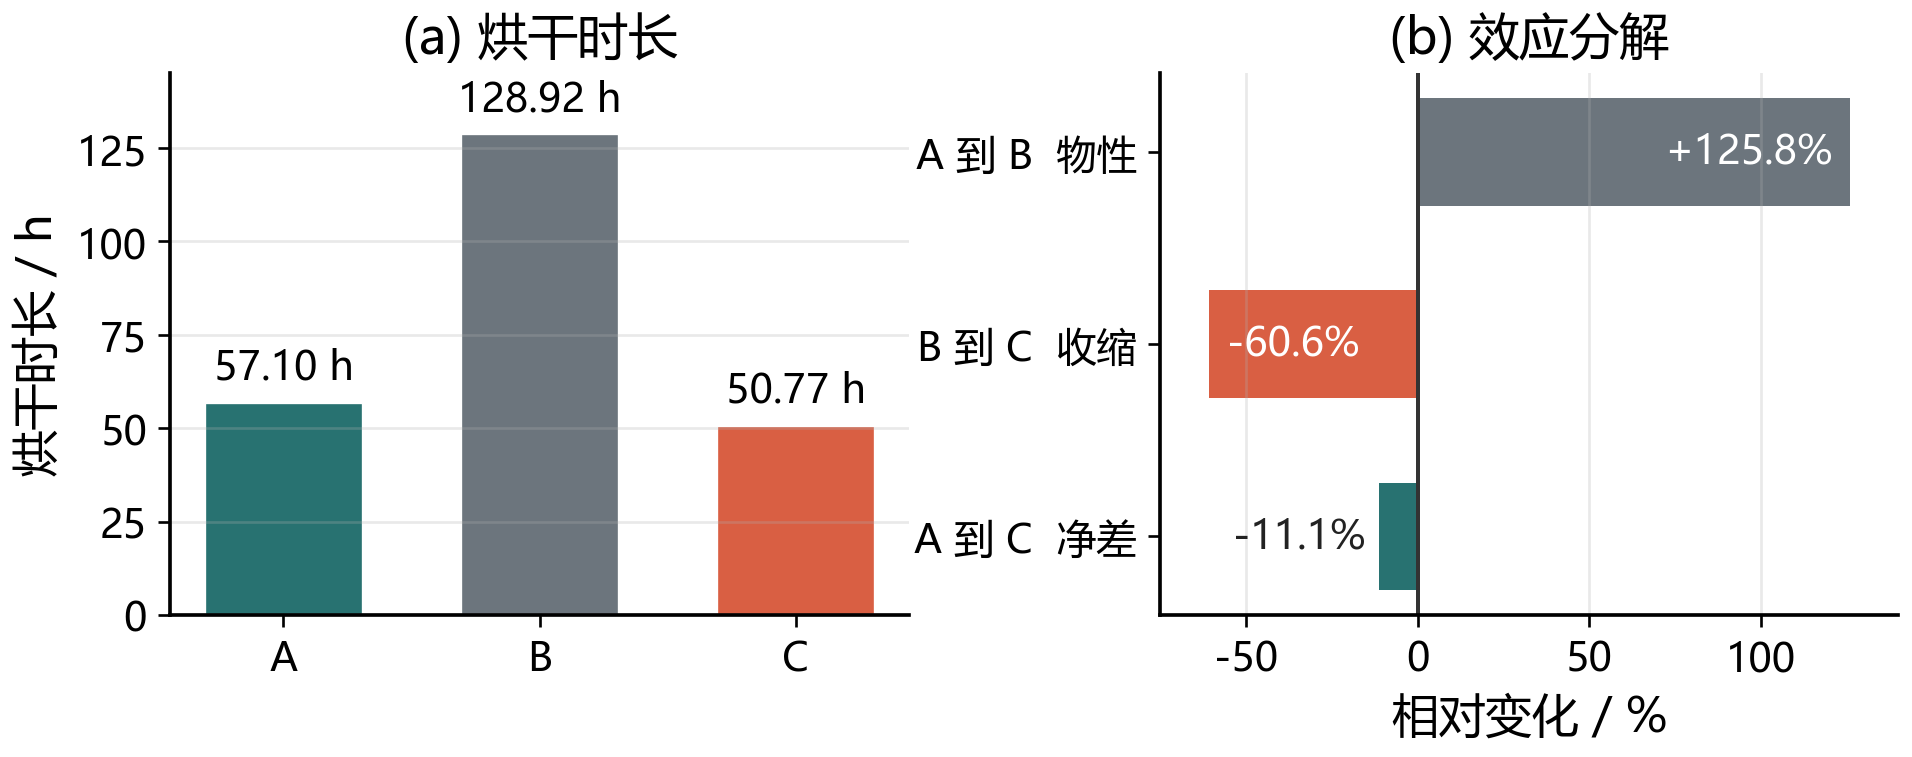
\includegraphics[width=0.86\textwidth]{fig20_p4_controlled.png}
\caption{三种受控场景的烘干时长及物性、收缩效应分解}
\label{fig:p4cmp}
\end{figure}

% =====================================================================
\section{数值方法}
\label{sec:numeric}

本节按 \S\ref{sec:reg} 给出的正则化坐标 $u=\xi^2$ 展开：先说明离散格式，
再交代时间积分与输出采样。

\subsection{Chebyshev--Gauss--Lobatto 谱配置}

取 $x_j=\cos(j\pi/N)$，$u_j=(1-x_j)/2\in[0,1]$，使 $u_0=0$、$u_N=1$。
标准 Chebyshev 微分矩阵由
\[
(D_x)_{ij}=\frac{c_i}{c_j}\frac{(-1)^{i+j}}{x_i-x_j}\ (i\ne j),\quad
(D_x)_{ii}=-\sum_{j\ne i}(D_x)_{ij},\quad
c_0=c_N=2,\ c_j=1
\]
给出；因 $u=(1-x)/2$，有 $D_u=-2D_x$。该构造是谱配置法处理边值问题的标准做法\cite{trefethen}。

\subsection{通量形式的配置}

把式 \eqref{eq:gov} 写成通量散度形式。记节点通量 $g_j^{(C)}=u_jD_j(D_uC)_j$，
内部节点用谱微分给出的通量，\textbf{表面通量直接取自 Robin 物理条件} \eqref{eq:bc_u}：
$g_N^{(C)}=\frac12h_mR(C_{\rm air}-C_N)$，于是
\begin{equation}
\frac{{\rm d}C_j}{{\rm d}t}=\frac{4}{R^2}\left(D_u\mathbf{g}^{(C)}\right)_j,
\qquad j=0,\dots,N.
\end{equation}
温度通量为 $g_j^{(T)}=u_jk_j(D_uT)_j$，表面取
$g_N^{(T)}=\frac12hR(T_{\rm air}-T_N)$，半离散方程明确写为
\begin{equation}
\frac{{\rm d}T_j}{{\rm d}t}
=\frac{4}{R^2\rho(C_j)c_p(C_j)}
\left(D_u\mathbf{g}^{(T)}\right)_j,
\qquad j=0,\dots,N.
\end{equation}

\begin{remark}[为何这种「混合通量」仍是谱精度]
$\mathbf g$ 在除 $u_N$ 外的节点上是插值多项式导数产生的通量，在 $u_N$ 上取物理边界通量
（解收敛时两者相等）。$\mathbf g$ 因而逐点收敛到真通量 $g(u)$，
谱微分 $D_u\mathbf g$ 在 $u_N$ 处谱收敛到 $g'(1)$；$u=0$ 处 $u_0=0$ 使 $g_0\equiv0$
自动满足对称性。\S\ref{sec:verify} 的数值实验确认了这一论证。
\end{remark}

\subsection{时间积分与输出采样}

时间方向采用变阶变步长隐式 BDF，物性在每个右端项求值处按当前状态重新计算
（而非冻结在上一步）。生产设置：$N=64$、$\mathrm{rtol}=10^{-11}$、
$\mathrm{atol}_C=10^{-13}$、$\mathrm{atol}_T=10^{-11}$；另用 Radau 与 LSODA 交叉验证。
输出用 CGL 节点上的重心插值
\[
C(u_*)=\frac{\sum_j\frac{w_j}{u_*-u_j}C_j}{\sum_j\frac{w_j}{u_*-u_j}},
\qquad w_j=(-1)^j\delta_j\ (\delta_0=\delta_N=\tfrac12,\ \delta_j=1),
\]
数值稳定且与插值多项式等价\cite{berrut}。烘干时长用自适应积分器的终端事件机制，
由稠密输出做 Brent 求交，不假设任何收敛阶。

% =====================================================================
\section{模型检验}
\label{sec:verify}

本章按「解析验证 $\to$ 多方法互证 $\to$ 残差统计 $\to$ 收敛性 $\to$ 稳定性 $\to$ 守恒性」
的顺序逐层检验。

\subsection{解析解验证：谱配置法对闭式解}

问题 1 的温度场有闭式解式 \eqref{eq:Tsol}，可作为\textbf{绝对基准}。
固定时间容差 $10^{-12}$、只加密空间，比较结果如表~\ref{tab:spec}。

\begin{table}[!ht]
\centering
\small
\caption{谱配置法与闭式解的比较（问题 1 温度场，$t=1800$ s）}
\label{tab:spec}
\begin{tabular}{@{}lcccccc@{}}
\toprule
$N$ & 4 & 6 & 8 & 12 & 24 & 64 \\
\midrule
全场最大误差 / K & $2.6\times10^{-10}$ & $1.3\times10^{-10}$ & $1.09\times10^{-10}$ &
$1.11\times10^{-10}$ & $1.14\times10^{-10}$ & $1.14\times10^{-10}$ \\
\bottomrule
\end{tabular}
\end{table}

误差在 $N=8$ 就已落到\textbf{时间积分误差平台}上并\textbf{不再随 $N$ 下降}——
这正是谱精度成立的标志（若边界通量处理有误，$N$ 增大也不会收敛）。
时间方向对应数据：$\mathrm{rtol}=10^{-8}$ 时误差 $1.0\times10^{-7}$ K、
$10^{-10}$ 时 $2.3\times10^{-9}$ K、$10^{-12}$ 时 $1.1\times10^{-10}$ K
（图~\ref{fig:besselval}）。

\begin{figure}[!ht]
\centering

\includegraphics[width=\textwidth]{fig11_bessel_validate.png}
\caption{谱收敛性曲线与偏差沿半径的分布}
\label{fig:besselval}
\end{figure}

\subsection{多方法互证：三种独立路线}

\begin{table}[!ht]
\centering
\small
\caption{三条相互独立的路线互证（问题 1）}
\begin{tabular}{@{}lccc@{}}
\toprule
量 & A：闭式解析解 & B：谱配置法（本文） & C：均匀网格守恒型有限体积 \\
\midrule
$T(0,1800)$ & 34.0424989 & 34.042499 & 34.042498 \\
$T(R_0,1800)$ & 37.1989220 & 37.198922 & 37.198921 \\
$C(R_0,1800)$ & --- & 1.51091810 & 1.51091918 \\
$C(R_0,1200)$ & --- & 1.65914239 & 1.65914441 \\
\bottomrule
\end{tabular}
\end{table}

路线 C 采用与 A、B 都不同的技术：均匀 $r$ 网格、守恒型有限体积、
等步长后向 Euler + Picard 迭代并在 $\Delta t\to0$ 上做 Richardson 外推
（外推法的原始文献见 \cite{richardson}）。
三法互差不超过 $2\times10^{-6}$。另在问题 2 的早时段（$t=0.5$ h、$r=0$）与
第三族对照格式（节点中心 FV $+\ \theta$ 法）比对：谱解 $32.565670279$，
对照格式一阶外推 $32.565670347$，两者相差 $6.8\times10^{-8}\,^\circ$C
（图~\ref{fig:three}）。三族方法互证说明：三者解的是同一个 PDE，
且各自离散误差均已被压到目标精度以下。

\begin{figure}[!ht]
\centering

\includegraphics[width=\textwidth]{fig21_three_methods.png}
\caption{三族离散的互证与精度量级对比}
\label{fig:three}
\end{figure}

\subsection{残差统计特性}

把 $N=64$ 的谱解与闭式解逐点相减，得到残差序列（共 $201$ 个空间点）。
如图~\ref{fig:resid} 所示，残差量级为 $10^{-10}$ K，且全部落在
$7.1\times10^{-11}\sim1.14\times10^{-10}$ K 的窄带内。
需要明确的是，这 $201$ 个残差\textbf{全部同号}（Shapiro--Wilk 检验
$p\approx3\times10^{-12}$），因此它们\textbf{不是}随机舍入噪声，而是时间积分器
留下的\textbf{确定性离散偏差}；其幅值随 $N$ 增大不再下降（表~\ref{tab:spec} 中
$N\ge8$ 后稳定在 $10^{-10}$ K 量级），说明空间方向已达谱精度、误差被时间积分平台接管。
故这里能支持的结论是「空间离散没有残留的模型失配信号」，
而\textbf{不能}据此断言残差服从正态分布。

\begin{figure}[!ht]
\centering

\includegraphics[width=\textwidth]{fig24_residual_qc.png}
\caption{谱解与闭式解偏差的直方图与 Q-Q 图（偏差为确定性离散误差，非随机噪声）}
\label{fig:resid}
\end{figure}

附件 1 的拟合残差同样做了统计诊断（图~\ref{fig:envstat}）：温度残差标准差
$0.334\,^\circ$C、峰值残差 $0.96\,^\circ$C，直方图近似正态；
但 Q-Q 图两端轻微偏离、滞后一阶自相关达 $0.83$，说明除随机噪声外还存在
\textbf{形式失配的系统性偏差}——这构成 \S\ref{sec:sens} 中环境口径灵敏度分析的动机。

\begin{figure}[!ht]
\centering

\includegraphics[width=\textwidth]{fig03_env_resid_stat.png}
\caption{附件 1 拟合残差的直方图与 Q-Q 图（上：温度；下：含湿量）}
\label{fig:envstat}
\end{figure}

\begin{figure}[!ht]
\centering

\includegraphics[width=\textwidth]{fig02_env_resid_time.png}
\caption{附件 1 拟合残差的时序（可见明显的系统失配区间）}
\label{fig:envresid}
\end{figure}

\subsection{收敛性分析}

\textbf{空间收敛}（图~\ref{fig:conv}(a)）：$t_{\rm dry}$ 随 $N$ 的变化为
$205557.9\to205565.2\to205572.3\to205574.5\to205575.4\to205575.5$ s
（$N=24,32,48,64,96,128$），$N=64$ 后变化已小于 $1$ s，
$N=96\to128$ 仅变 $0.1$ s，故取连续极限 $205575.5$ s。
本节的空间/时间扫描数据由脚本 \texttt{verify\_data.py} 复跑产生并存入
\texttt{中间数据/verification.json}，图~\ref{fig:conv} 直接读该文件，
绘图前会强制校验数据与解缓存一致（不一致即报错，不画图）。

\textbf{报告值与交付文件的口径}：正文报告的 $205575.5$ s 是 $N=128$ 的连续极限值，
而 \texttt{result3.xlsx} 按生产设置 $N=64$ 生成，其终点为 $205574.5$ s，
两者相差 $1.0$ s（相对差 $5\times10^{-6}$）。这一差异正是上表所列的空间离散误差，
属同一模型的两种网格口径，不是两个不同结果。同理，\S\ref{sec:shrink} 表~\ref{tab:p4control}
的 A 行取连续极限值，B、C 两行取 $N=64$ 的生产值，B 行另给出 $N=48$ 的复算值 $464118.2$ s
以说明该行差异确属网格误差；表~\ref{tab:sens} 的灵敏度基准取 $N=64$。

\textbf{时间收敛}（图~\ref{fig:conv}(b)）：作为对照，用常见的节点中心有限体积
$+\ \theta$ 法（CN、前 4 步 Rannacher 启动、物性冻结于上一时间步）在 $N=1600$ 下
计算烘干时长并改变步长，结果如表~\ref{tab:dt}。

\begin{table}[!ht]
\centering
\small
\caption{定步长 $\theta$ 法的时间收敛性（问题 3，$N=1600$）}
\label{tab:dt}
\begin{tabular}{@{}lccccccc@{}}
\toprule
$\Delta t$ / s & 40 & 20 & 10 & 5 & 2 & 1 & 0.5 \\
\midrule
$t_{\rm dry}$ / s & 205508.5 & 205538.7 & 205553.8 & 205561.3 & 205565.9 & 205567.4 & 205568.1 \\
相邻增量 / s & --- & 30.2 & 15.1 & 7.5 & 4.5 & 1.5 & 0.7 \\
\bottomrule
\end{tabular}
\end{table}

$\Delta t$ 每减半、增量近似减半，是严格的 $\mathcal{O}(\Delta t)$ \textbf{一阶}收敛：
把相邻增量与步长的几何中点取双对数，拟合斜率为 $1.01$（一阶应取 $1$）。
用最细三档步长对 $t(\Delta t)=L-c\Delta t$ 做最小二乘得 $c\approx1.42$ s$/$s，
外推得该格式极限 $205568.8$ s，
再加空间 Richardson 极限与时间修正后回到 $205575.5$ s，与本文谱解一致。
一阶误差的来源是物性冻结于上一时间步，使实际推进只有 $\mathcal{O}(\Delta t)$ 相容。
\textbf{若在长时间段放宽步长（如取 $\Delta t=10$ s 以节省计算量），
仅此一项就会把烘干时长系统性低估约 $15$ s（相对偏差 $0.008\%$）。}

\begin{figure}[!ht]
\centering

\includegraphics[width=\textwidth]{fig22_convergence.png}
\caption{时间步收敛（严格一阶）与空间收敛（谱解远快于二阶）}
\label{fig:conv}
\end{figure}

\subsection{时间积分器与容差的稳定性}

为避免单一积分器带来的偶然性，对问题 3 换积分器与容差重算：

\begin{table}[!ht]
\centering
\small
\caption{烘干时长对时间积分器与容差的不敏感性（问题 3）}
\label{tab:integ}
\begin{tabular}{@{}lcccccc@{}}
\toprule
配置 & BDF $10^{-9}$ & BDF $10^{-10}$ & BDF $10^{-12}$ & Radau $10^{-11}$ & LSODA $10^{-10}$ & 1 s 密采样求交 \\
\midrule
$t_{\rm dry}$ / s & 205574.525 & 205574.519 & 205574.518 & 205574.518 & 205574.519 & 205574.519 \\
\bottomrule
\end{tabular}
\end{table}

表~\ref{tab:integ} 中六种积分器与容差配置（3 族积分器 $\times$ 4 个容差，
另加 1 s 密采样求交）的极差仅 $0.007$ s（图~\ref{fig:integ}）；
「终端事件求交」与「1 s 密采样 $+$ 线性求交」给出完全相同的值（差 $0.000$ s），
说明事件定位本身没有引入误差。该时刻 $\mathrm{d}C_0/\mathrm{d}t=-2.94\times10^{-7}$ s$^{-1}$，
即 $1$ s 的定位误差仅对应 $2.9\times10^{-7}$ kg/kg 的浓度误差。

\begin{figure}[!ht]
\centering

\includegraphics[width=\textwidth]{fig23_integrator.png}
\caption{时间积分器与容差稳定性：全部配置的极差为 $0.007$ s}
\label{fig:integ}
\end{figure}

\subsection{守恒性检验}
\label{sec:cons}

固定半径时，单位长度药材的水分质量和截面面积平均含水率分别为
\[
M_w(t)=\pi\rho_dR_0^2\int_0^1C(u,t)\,{\rm d}u,
\qquad
\bar C(t)=\int_0^1C(u,t)\,{\rm d}u.
\]
由式 \eqref{eq:mass} 与 Robin 边界可得
\begin{equation}
\frac{{\rm d}M_w}{{\rm d}t}
=-2\pi R_0\rho_dh_m(C_s-C_{\rm air}).
\label{eq:masscheck}
\end{equation}
问题 4 中 $\rho_dR(t)^2=\rho_{d0}R_0^2$，故同一校核仍成立，只需把边界周长改为
$2\pi R(t)$。数值上用高阶求积计算式 \eqref{eq:masscheck} 两侧，检验总量变化与表面流出量的一致性。
原先的 $\int_0^1 2uC\,{\rm d}u$ 不是圆柱截面的面积平均量，现已改为上述正确表达。
本文所有以「截面平均」报出的数字（问题一与问题三的结果分析，以及图~\ref{fig:p3}(b) 的
$\bar C$ 曲线）一律按 $\bar C=\int_0^1C\,{\rm d}u$ 计算；
实现上先由 Gauss--Legendre 求积把 Lagrange 基函数的积分算成一组固定权重，
再用权重与节点值的内积逐时刻取值，故不依赖任何采样点数的选取。

% =====================================================================
\section{灵敏度与不确定度分析}
\label{sec:sens}

本章的灵敏度分析均由脚本 \texttt{sensitivity.py} 重新求解，
共 $12$ 组参数扰动，指标为问题 3 的烘干时长 $t_{\rm dry}$。
\textbf{基准口径}：基准解取 $N=64$（与 \texttt{result3.xlsx} 的生产网格一致）、
附录 3 物性与一阶惯性拟合环境，$t_{\rm dry}=205574.5$ s；
表中所有相对变化都以该基准为分母。改用连续极限 $205575.5$ s 作分母
只会把各相对变化改变 $5\times10^{-6}$，不影响排序与量级。

\subsection{参数扰动结果}

\begin{table}[!ht]
\centering
\small
\caption{关键参数扰动对烘干时长的影响（基准：$N=64$，$t_{\rm dry}=205574.5$ s）}
\label{tab:sens}
\begin{tabular}{@{}lccc@{}}
\toprule
扰动 & $t_{\rm dry}$ / s & 相对变化 & 绝对变化 / s \\
\midrule
$E$ $+2\%$（$3850\to3927$ K） & 254624.0 & $+23.86\%$ & $+49050$ \\
$E$ $-2\%$（$3850\to3773$ K） & 167355.9 & $-18.59\%$ & $-38219$ \\
$a$ $+2\%$（$0.45\to0.459$） & 215664.2 & $+4.91\%$ & $+10090$ \\
$a$ $-2\%$（$0.45\to0.441$） & 196057.7 & $-4.63\%$ & $-9517$ \\
$D_0$ $-2\%$ & 209277.8 & $+1.80\%$ & $+3703$ \\
$D_0$ $+2\%$ & 202019.9 & $-1.73\%$ & $-3555$ \\
$T_{\rm set}$ $-0.2$ K & 206911.0 & $+0.65\%$ & $+1336$ \\
$T_{\rm set}$ $+0.2$ K & 204250.0 & $-0.64\%$ & $-1325$ \\
$h_m$ $-2\%$ & 206055.5 & $+0.23\%$ & $+481$ \\
$h_m$ $+2\%$ & 205116.3 & $-0.22\%$ & $-458$ \\
$h$ $-2\%$ & 205580.3 & $+0.003\%$ & $+6$ \\
$h$ $+2\%$ & 205569.0 & $-0.003\%$ & $-6$ \\
\bottomrule
\end{tabular}
\end{table}

表~\ref{tab:sens}的扰动口径如下，以免误读：$E$、$a$、$D_0$ 三项只改物性式中的对应因子；
$h$、$h_m$ 只改传递系数；$T_{\rm set}$ 只是把烘房设定值平移
$\pm0.2$ K——因一阶惯性式的初值锚定在实测的 $T_{\rm air}(0)=28\,^\circ$C 上，
初始环境温度不受影响，被扰动的是设定值与整条升温轨迹。

\textbf{主导不确定性的参数是活化温度 $E$}：$\pm2\%$ 使 $t_{\rm dry}$ 变化
$+23.9\%$ / $-18.6\%$。该响应明显不对称，
升温方向的敏感性更强，这是 Arrhenius 因子 $e^{-E/T_K}$ 的非线性所致
（$E$ 增大时 $D$ 的下降在低温段更快，而干燥前期温度较低）。
活化浓度指数 $a$ 次之（$\pm2\%$ 约 $\pm4.8\%$）；
$D_0$、$T_{\rm set}$、$h_m$ 的影响都在 $2\%$ 以内；
而对流换热系数 $h$ 的影响小于 $0.01\%$——因为温度在 $2$ h 内即达到准平衡，
$h$ 只影响升温的快慢，不影响后期的准等温干燥速率。

\subsection{解析局部灵敏度对照}

对 $D=D_0e^{-a/C}e^{-E/T_K}$ 取对数，有
$\ln D=\ln D_0-a/C-E/T_K$，故
\begin{equation}
\frac{\partial\ln D}{\partial T_K}=\frac{E}{T_K^2},\qquad
\frac{\partial\ln D}{\partial a}=-\frac{1}{C},\qquad
\frac{\partial\ln D}{\partial C}=\frac{a}{C^2}.
\end{equation}
在 $T_K=323.15$ K（$50\,^\circ$C）处，$\partial\ln D/\partial T_K
=3.69\times10^{-2}$ K$^{-1}$，表示其他变量局部不变时，温度偏差 $1$ K 使 $D$ 约变化 $3.7\%$。
这一局部导数不能直接替代全程烘干时长的扰动重算。
在 $C=0.15$ kg/kg、$a=0.45$ 附近，$\partial\ln D/\partial a=-6.67$，
$a$ 增加 $2\%$ 即 $\Delta a=0.009$ 时，线性近似给出 $\Delta\ln D\approx-0.060$，
即局部 $D$ 约下降 $5.8\%$；同时 $\partial\ln D/\partial C=20.0$ (kg/kg)$^{-1}$。
该数量级与表中全模型重算所显示的后期敏感性相符。

\subsection{环境口径的灵敏度}

附件 1 的拟合残差存在系统性失配（图~\ref{fig:envresid}），
故必须评估「如何把实测序列转成边界条件」这一建模选择的影响。
两种口径的对比结果如表~\ref{tab:ambient}。
\textbf{口径约定}：「原始序列插值」把温度与含湿量\textbf{同时}换回附件 1 的实测序列
线性插值（而不是只换温度）；$t>14400$ s 后两者都取各自的设定值。

\begin{table}[!ht]
\centering
\small
\caption{环境口径对结果的影响（基准网格 $N=64$）}
\label{tab:ambient}
\begin{tabular}{@{}lcccc@{}}
\toprule
环境口径 & $T(0,1800)$ / $^\circ$C & $T(R_0,1800)$ / $^\circ$C & $C(R_0,1800)$ & $t_{\rm dry}$ / s \\
\midrule
一阶惯性拟合（本文） & 34.0425 & 37.1989 & 1.5109 & 205574.5 \\
附件 1 原始序列插值 & 33.5753 & 36.7856 & 1.5102 & 205578.9 \\
\midrule
差值 & $-0.467$ & $-0.413$ & $-0.0007$ & $+4.4$ \\
\bottomrule
\end{tabular}
\end{table}

\textbf{这是一个重要且反直觉的结论}：环境口径对问题 1 的温度场影响高达
$0.467\,^\circ$C（比所有数值误差之和大三个数量级），但对烘干时长的影响
只有 $+4.4$ s（$0.002\%$）。原因是 $t_{\rm dry}$ 由长达 $50$ h 以上的恒温干燥段决定，
而两种口径在该段的差异随 $e^{-t/\tau_T}$ 迅速衰减至零；
反之前 $30$ min 的预热段正是环境口径差异最大的区间，
故对问题 1 影响显著而对问题 3 几乎无影响。
注意温度场的差异与含湿量口径无关：问题 1 中两场解耦，
故切换 $C_{\rm air}$ 不改变 $T(0,1800)$ 与 $T(R_0,1800)$。

\subsection{不确定度汇总}

综合来看，本题结果的不确定度\textbf{不是由数值方法决定的}
（数值误差 $<0.01\%$），而是由以下三项决定，按贡献排序：

\begin{enumerate}[leftmargin=1.9em,itemsep=2pt]
\item \textbf{物性经验式的标定精度}（主导）。$E=3850$ K 只要偏差 $1\%$ 就会使
$t_{\rm dry}$ 变化约 $10\%$；而该参数由题目附录直接给定，无法由题面数据进一步校验。
\item \textbf{环境口径}（次要，且只影响早时段）。对问题 1 温度场影响 $0.467\,^\circ$C，
对烘干时长影响 $0.002\%$。
\item \textbf{未建模的物理机制}（无法定量）。主要是表面蒸发潜热引起的降温，
题目未提供汽化潜热与孔隙率，无法标定。
\end{enumerate}

% =====================================================================
\section{模型的评价与推广}
\label{sec:eval}

\subsection{模型优点}

\textbf{方法与精度方面}，变换 $u=(r/R)^2$ 将圆柱轴心正则化并使谱配置可用；
问题 1 的常物性温度场在 $N=8$ 时误差已达 $10^{-10}$ 量级，非线性问题则依据网格加密选取
$N=64$。准静态分解还给出 Bessel 闭式解，在本文验证时刻保留前 $2$ 项即可达到机器精度。

\textbf{验证与解释方面}，闭式解、谱配置法和两族有限体积格式的互差不超过
$2\times10^{-6}$，且同时核验守恒性、收敛阶、积分器与容差稳定性；对事件时刻的一阶离散误差
作了专门量化。实际扰动试验识别出 $E$ 与 $a$ 为主导参数，并以受控对照拆分物性变化与纯收缩效应，
避免把跨问题净差异误判为单一几何因素。

\subsection{模型缺点}

模型的主要限制依次为：\textbf{物性标定不足}，主导参数 $E$、$a$ 只能取自附录，宜以恒温薄层
实验复核；\textbf{蒸发潜热缺失}，可能高估温度和扩散率；\textbf{热梯度驱动的水分迁移}未显式建模，
该机制可产生额外水分通量\cite{philip}；\textbf{各向同性仿射收缩}，不能描述
非仿射或各向异性变形；\textbf{一维径向简化}，忽略端面对流与轴向梯度；\textbf{经验式外推风险}，
题面未给出 $D(C,T)$ 的标定区间，故在 $C\to0.15$ 附近仍需实验验证。

\subsection{改进方向与推广}

后续可用加热功率与排湿速率建立闭环烘房模型，以替代式 \eqref{eq:ambient}；获得含湿焓、
汽化潜热和界面相平衡数据后，可改用焓方程描述蒸发冷却。对球体仍可取 $u=\xi^2$，但须重新推导
球坐标算子；平板无轴心奇异项，不必照搬该变换。谱配置框架可迁移至药物颗粒、食品和木材等体系，
也可将阈值事件替换为有效成分保留率等目标；本文针对事件时刻的双格式误差核验方法同样可复用。
就工艺本身而言，本文给出的「收缩使烘干时长缩短 $60.6\%$」这一量级说明：按固定几何标定的
工艺参数在中后期会系统性偏保守，分段温湿度等主动调控策略\cite{ju2019stepdown}值得进一步研究。

% =====================================================================
\noindent\textbf{AI工具使用声明。}本参赛队在竞赛过程中使用了 AI 工具，主要用于候选模型比较、论文结构整理、语言润色、
公式一致性检查与图表排版建议。模型方程、数值结果和结论均依据题目数据与可运行程序复核，
详细使用情况见支撑材料《AI工具使用详情.pdf》。

% =====================================================================
\begin{thebibliography}{99}
% 字号：原为 \scriptsize（本模板下实为 6.5 pt = 小六），不足正文字号的一半，英文
% 条目在纸质版上难以正常阅读。改为 \normalsize（小四 12.05 pt），与正文同号——
% 与工作区里那份同题示范论文的做法一致，且实测不增加页数。
\normalsize
% 条目之间留一点空隙：字号变大后 0 pt 的间距会让相邻条目糊成一段。
\setlength{\itemsep}{1.5pt plus 0.5pt}
\setlength{\parskip}{0pt}
\bibitem{hussain} Hussain M M, Dincer I. Two-dimensional heat and moisture transfer
analysis of a cylindrical moist object subjected to drying: A finite-difference approach.
International Journal of Heat and Mass Transfer, 2003, 46(21): 4033--4039.
\bibitem{wang1995} Wang N, Brennan J G. A mathematical model of simultaneous heat and
moisture transfer during drying of potato. Journal of Food Engineering, 1995, 24(1): 47--60.
\bibitem{ao2026modeling} Ao J, He W, Chen Y, Ai Z, Li T, Xiao H, Xiao Z. Modeling and
analysis of heat and moisture transfer during \textit{Fructus aurantii} drying based on
CT scanning. Drying Technology, 2026, 44(8): 1183--1196.
\bibitem{ju2019stepdown} Ju H-Y, Zhao S-H, Mujumdar A S, Zhao H-Y, Duan X, Zheng Z-A,
Gao Z-J, Xiao H-W. Step-down relative humidity convective air drying strategy to enhance
drying kinetics, efficiency, and quality of American ginseng root
(\textit{Panax quinquefolium}). Drying Technology, 2019, 38(7): 903--916.
\bibitem{luikov} Luikov A V. Systems of differential equations of heat and mass transfer
in capillary-porous bodies (review). International Journal of Heat and Mass Transfer,
1975, 18(1): 1--14.
\bibitem{whitaker} Whitaker S. Simultaneous Heat, Mass, and Momentum Transfer in Porous
Media: A Theory of Drying. Advances in Heat Transfer, 1977, 13: 119--203.
\bibitem{zhangwp} 张卫鹏, 高振江, 肖红伟, 郑志安, 巨浩羽, 谢龙.
基于 Weibull 函数不同干燥方式下的茯苓干燥特性. 农业工程学报, 2015, 31(5): 317--324.
\bibitem{carslaw} Carslaw H S, Jaeger J C. Conduction of Heat in Solids. 2nd ed.
Oxford: Clarendon Press, 1959.
\bibitem{lewis} Lewis W K. The Rate of Drying of Solid Materials.
Journal of Industrial \& Engineering Chemistry, 1921, 13(5): 427--432.
\bibitem{trefethen} Trefethen L N. Spectral Methods in MATLAB.
Philadelphia: Society for Industrial and Applied Mathematics (SIAM), 2000.
\bibitem{berrut} Berrut J-P, Trefethen L N. Barycentric Lagrange Interpolation.
SIAM Review, 2004, 46(3): 501--517.
\bibitem{richardson} Richardson L F. IX. The approximate arithmetical solution by finite
differences of physical problems involving differential equations, with an application to
the stresses in a masonry dam. Philosophical Transactions of the Royal Society of London.
Series A, 1911, 210: 307--357.
\bibitem{philip} Philip J R, De Vries D A. Moisture movement in porous materials under
temperature gradients. Transactions, American Geophysical Union, 1957, 38(2): 222--232.
\end{thebibliography}

% =====================================================================
\newpage
\appendix

\section{Bessel--Duhamel 展开系数推导}
\label{app:besselcoef}

设 $\langle f,g\rangle=\int_0^Rrfg\,{\rm d}r$。函数 $W$ 与特征函数
$\phi_n$ 满足同一齐次 Robin 条件，因而 Green 恒等式的边界项为零：
\[
\int_0^Rr\left[(\nabla^2W)\phi_n-W(\nabla^2\phi_n)\right]{\rm d}r
=R\left[W'(R)\phi_n(R)-W(R)\phi_n'(R)\right]=0.
\]
再利用
$\nabla^2\phi_n=-(\beta_n^2/R^2)\phi_n$、
$\nabla^2W=\kappa^2(A-W)$，左端被积函数化为
$\kappa^2Ar\phi_n-\left[(\beta_n^2/R^2)-\kappa^2\right]rW\phi_n$，于是
\[
\kappa^2A\langle1,\phi_n\rangle
-\left[\frac{\beta_n^2}{R^2}-\kappa^2\right]\langle W,\phi_n\rangle=0
\quad\Longrightarrow\quad
\langle W,\phi_n\rangle
=-\frac{\kappa^2A}{(\beta_n^2/R^2)-\kappa^2}\langle1,\phi_n\rangle .
\]
\textbf{注意此处的负号}：$\hat w$ 的初值是 $-W(r)$，展开系数 $b_n$ 取的是 $-W$ 的
带权投影，故该负号在 $b_n$ 与 $\kappa^2$ 前的符号相消。代入
$\langle1,\phi_n\rangle=R^2J_1(\beta_n)/\beta_n$ 与
$\|\phi_n\|^2=\frac{R^2}{2}\left[J_0^2(\beta_n)+J_1^2(\beta_n)\right]$，得
\begin{equation}
b_n=\frac{\langle -W,\phi_n\rangle}{\|\phi_n\|^2}
=\frac{A\kappa^2N_n}{(\beta_n^2/R^2)-\kappa^2},
\qquad
N_n=\frac{2J_1(\beta_n)}{\beta_n\left[J_0^2(\beta_n)+J_1^2(\beta_n)\right]},
\label{eq:bn}
\end{equation}
即正文式~\eqref{eq:Tsol}中的 $b_n$。
本题所用参数与前四阶数值为
\[
\begin{aligned}
&\alpha=1.688555\times10^{-7}\ {\rm m^2/s},\quad R_0^2/\alpha=2368.89\ {\rm s},\quad
\mathrm{Bi}=1.388889,\quad \kappa R_0=1.123265,\\
&\beta_{1..4}=(1.4184725,4.1664696,7.2084785,10.3082732),\\
&b_{1..4}=(47.2789,-0.65803,0.096714,-0.027695).
\end{aligned}
\]

\section{支撑材料清单}

\begin{table}[!ht]
\centering
\footnotesize
\begin{tabular}{@{}p{1.4cm}p{4.4cm}p{8.9cm}@{}}
\toprule
类别 & 文件 & 说明 \\
\midrule
\multirow{12}{*}{源程序}
 & \texttt{common.py} & 参数、烘房环境标定、物性经验式、附件读取 \\
 & \texttt{spectral.py} & 主求解器：$u=\xi^2$ 谱配置 + 自适应 BDF \\
 & \texttt{analytic\_p1.py} & 问题 1 温度场 Bessel--Duhamel 闭式解 \\
 & \texttt{fv\_theta.py} & 对照格式：节点中心 FV + 定步长 $\theta$ 法 \\
 & \texttt{fv\_uniform.py} & 对照格式：均匀网格守恒型 FV + 后向 Euler \\
 & \texttt{run\_all.py} & 一键复跑全部结果与验证 \\
 & \texttt{make\_results.py} & 生成 result1--4.xlsx \\
 & \texttt{sensitivity.py} & 灵敏度分析（12 组扰动 + 环境口径分叉） \\
 & \texttt{verify\_data.py} & 复跑图 25/26 的收敛性与积分器数据，并做一致性校验 \\
 & \texttt{make\_figures.py}、\texttt{fig\_core.py} & 生成全部论文插图、绘图样式与解缓存 \\
 & \texttt{make\_controlled\_comparison.py} & 生成问题 4 受控对照图并复算固定半径基准 \\
 & \texttt{console\_utf8.py} & 控制台编码修复 \\
\midrule
\multirow{4}{*}{结果数据}
 & \texttt{result1.xlsx} & 问题 1 温度/水分浓度，$1800\times21$ \\
 & \texttt{result2.xlsx} & 问题 2 温度/水分浓度，$10800\times21$ \\
 & \texttt{result3.xlsx} & 问题 3 水分浓度，$3427\times21$（$N=64$，终点 $205574.5$ s） \\
 & \texttt{result4.xlsx} & 问题 4 水分浓度（含表面列），$3047\times22$ \\
\midrule
\multirow{3}{*}{中间数据}
 & \texttt{solutions.npz} & 四问的解缓存（含生成时的代码指纹，防止误用旧缓存） \\
 & \texttt{verification.json} & 图 25/26 的收敛性与积分器复跑数据 \\
 & \texttt{sensitivity.txt/.npz} & 灵敏度分析原始输出 \\
\midrule
附件数据 & \texttt{附件1.xlsx}、\texttt{附件2.xlsx} &
赛题给出的烘房环境与半径实测序列；虽属赛题原始数据，仍随包保留，
以便 \texttt{common.py} 按文件名自动定位附件、整包直接复跑 \\
\midrule
图表 & \texttt{fig01--fig26} &
论文插图 27 张 PNG（240 dpi 渲染，中文标签），其中 26 张被正文引用；
未采用的 \texttt{fig20\_p4\_vs\_p3.png} 不列入本清单（原因见下方说明） \\
AI 使用详情 & \texttt{AI工具使用详情.pdf} & AI 工具信息、使用环节与对输出的采纳情况 \\
\bottomrule
\end{tabular}
\end{table}

上表中 \texttt{fig20\_p4\_vs\_p3.png} 为何未采用：该图直接把问题 3 与问题 4 的
$t_{\rm dry}$ 相减，而这两个问题\textbf{同时}改变了物性关系与几何，其差值 $-11.1\%$
是二者共同作用的净结果，把它当作"收缩效应"属于错误归因。本文改用同一物性下仅改半径的
受控对照（表~\ref{tab:p4control}、图~\ref{fig:p4cmp}）来隔离收缩，纯收缩贡献为
$-60.6\%$。为避免被误引，该图不进入正文，也不列入本清单。

复跑方式（依赖 Python 3.9+ 与 numpy、scipy、openpyxl；其中
\texttt{make\_figures.py}、\texttt{make\_controlled\_comparison.py} 重绘插图还需
matplotlib $\ge 3.5$，其余脚本对 matplotlib 版本无要求）：
\begin{lstlisting}[language=bash]
python run_all.py              # 全部结果 + 全部验证，约 4-5 分钟
python make_results.py         # 重新生成 result1-4.xlsx（写入 result/）
python sensitivity.py          # 重新运行灵敏度分析
python verify_data.py --recompute   # 重建图 25/26 的验证数据（约 22 分钟）
python make_figures.py         # 重新生成全部插图（写入 figure/）
\end{lstlisting}
\texttt{common.py} 会在包内目录树中自动搜索附件路径，整个包可直接移动位置后运行。
\texttt{make\_figures.py} 会先校验 \texttt{verification.json} 与解缓存是否一致，
不一致即中止并提示重建，避免画出与代码结果脱钩的图。

% =====================================================================
\section{完整源程序代码}

\subsection{公共参数与环境标定：\texttt{common.py}}
\lstinputlisting[language=Python]{../code/common.py}

\subsection{主求解器：\texttt{spectral.py}}
\lstinputlisting[language=Python]{../code/spectral.py}

\subsection{问题 1 温度场闭式解：\texttt{analytic\_p1.py}}
\lstinputlisting[language=Python]{../code/analytic_p1.py}

\subsection{对照格式一：节点中心有限体积 $+\ \theta$ 法：\texttt{fv\_theta.py}}
\lstinputlisting[language=Python]{../code/fv_theta.py}

\subsection{对照格式二：均匀网格守恒型有限体积：\texttt{fv\_uniform.py}}
\lstinputlisting[language=Python]{../code/fv_uniform.py}

\subsection{一键复跑全部结果与验证：\texttt{run\_all.py}}
\lstinputlisting[language=Python]{../code/run_all.py}

\subsection{结果文件生成：\texttt{make\_results.py}}
\lstinputlisting[language=Python]{../code/make_results.py}

\subsection{灵敏度分析：\texttt{sensitivity.py}}
\lstinputlisting[language=Python]{../code/sensitivity.py}

\subsection{绘图基础模块：\texttt{fig\_core.py}}
\lstinputlisting[language=Python]{../code/fig_core.py}

\subsection{论文插图生成：\texttt{make\_figures.py}}
\lstinputlisting[language=Python]{../code/make_figures.py}

\subsection{问题 4 受控对照：\texttt{make\_controlled\_comparison.py}}
\lstinputlisting[language=Python]{../code/make_controlled_comparison.py}

\subsection{验证数据复跑与一致性校验：\texttt{verify\_data.py}}
\lstinputlisting[language=Python]{../code/verify_data.py}

\subsection{控制台编码修复：\texttt{console\_utf8.py}}
\lstinputlisting[language=Python]{../code/console_utf8.py}

\end{document}


